\documentclass[12pt,a4paper, usenames, dvipsnames]{article}
\usepackage{graphicx}
\usepackage{xcolor}


\usepackage[ngerman]{babel}
\usepackage[utf8]{inputenc}
\usepackage{mathtools}
\usepackage{amsmath}
\usepackage{amssymb}
\usepackage{geometry}
\usepackage{scrpage2}
\usepackage{tikz}
\usepackage{float}
\usepackage{verbatim}

\usepackage{ stmaryrd }

\usepackage{subfigure}

\usepackage[compact]{titlesec}     


\usepackage[center]{caption}


\pagestyle{plain}


\usepackage[backend=bibtex,style=numeric, citestyle = numeric]{biblatex}

\bibliography{references.bib}






\geometry{
  paper=a4paper, % Change to letterpaper for US letter
  top=3cm, % Top margin
  left=2cm, % Left margin
  right=3cm, % Right margin
  %showframe, % Uncomment to show how the type block is set on the page
}

\setlength{\parindent}{0em}

\pagenumbering {arabic} 

\titlespacing*{\section}{0pt}{10ex plus 1ex minus .2ex}{4.3ex plus .2ex}









\begin{document}




\begin{titlepage}
	\centering
	{\scshape\LARGE Technische Universität Dortmund \par}
	Fakultät für Informatik \par
	Lehrstuhl 14 für Software Engineering \par
	\vspace{1cm}
	{\scshape\Large Bachelorarbeit \par }
	\vspace{1.5cm}
	{\huge\bfseries  Gruppentheorie des 2x2x2 Zauberwürfels und dessen Lösungsalgorithmen \par}
	\vspace{2cm}
	{\Large\itshape Pina Kolling\par}
	\vspace{0.5cm}
	{Abgabe: Mai 2021 \par }
	\vfill
	betreut von\par
	Dr. Lukasz \textsc{Czajka} \par 
	und \par 
	M. Sc. Christoph \textsc{Stahl} 

	\vfill

% Bottom of the page
	{\large \today\par}
\end{titlepage}


\tableofcontents

\thispagestyle{empty} 



\newpage

\setcounter{page}{1} 









%=======================================================================================================










\section{Einleitung/Ausgangslage}

Meine Bachelorarbeit befasst sich mit dem 2x2x2 Zauberwürfel und dessen Algorithmen zur Lösung. Dabei handelt es sich um ein Drehpuzzle, das ein mathematisches Problem darstellt. \\ 
Im Folgenden werde ich die Terminologie und den Aufbau des Würfels erklären.\\
Terminologie:
\begin{figure}[h]
\centering
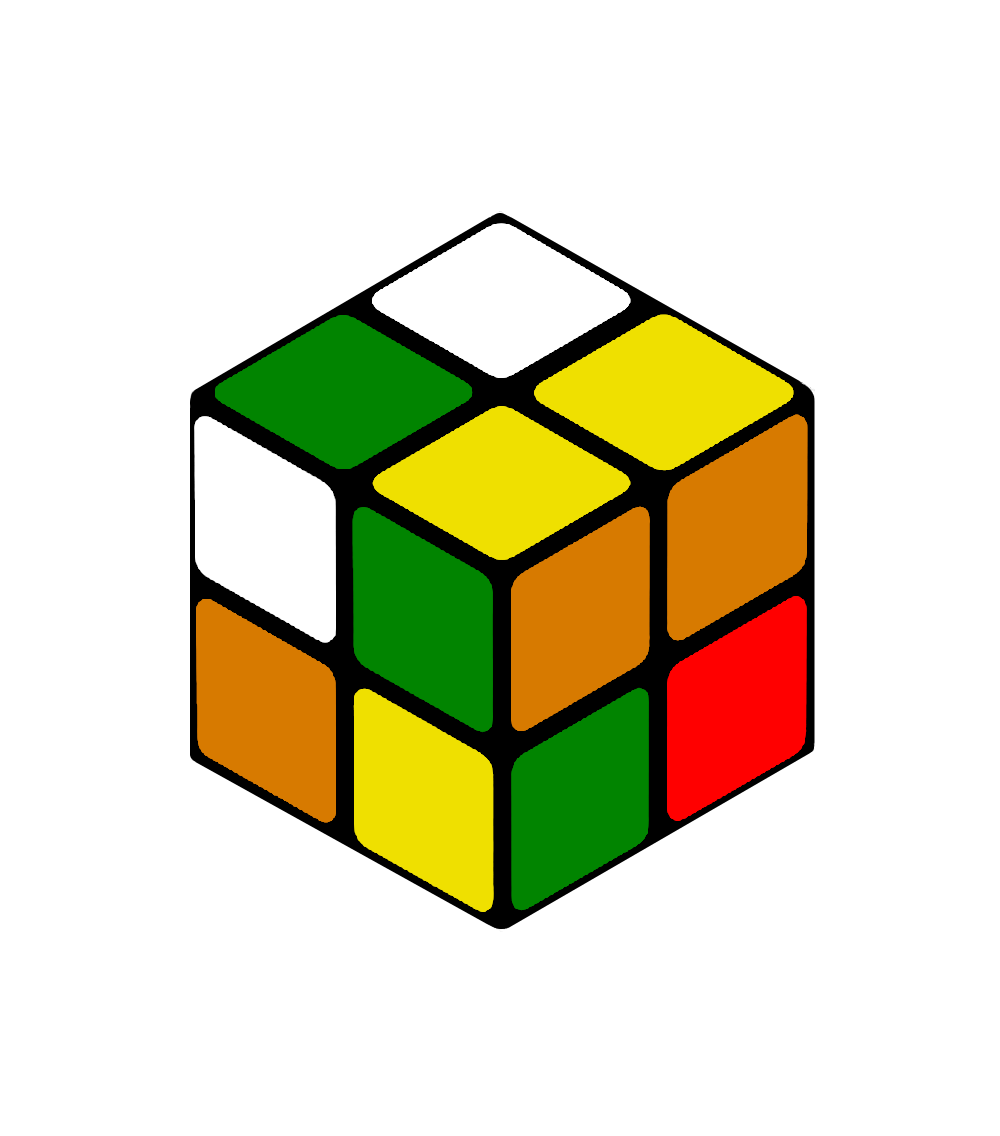
\includegraphics[scale=0.1]{2x2scrambled.png}
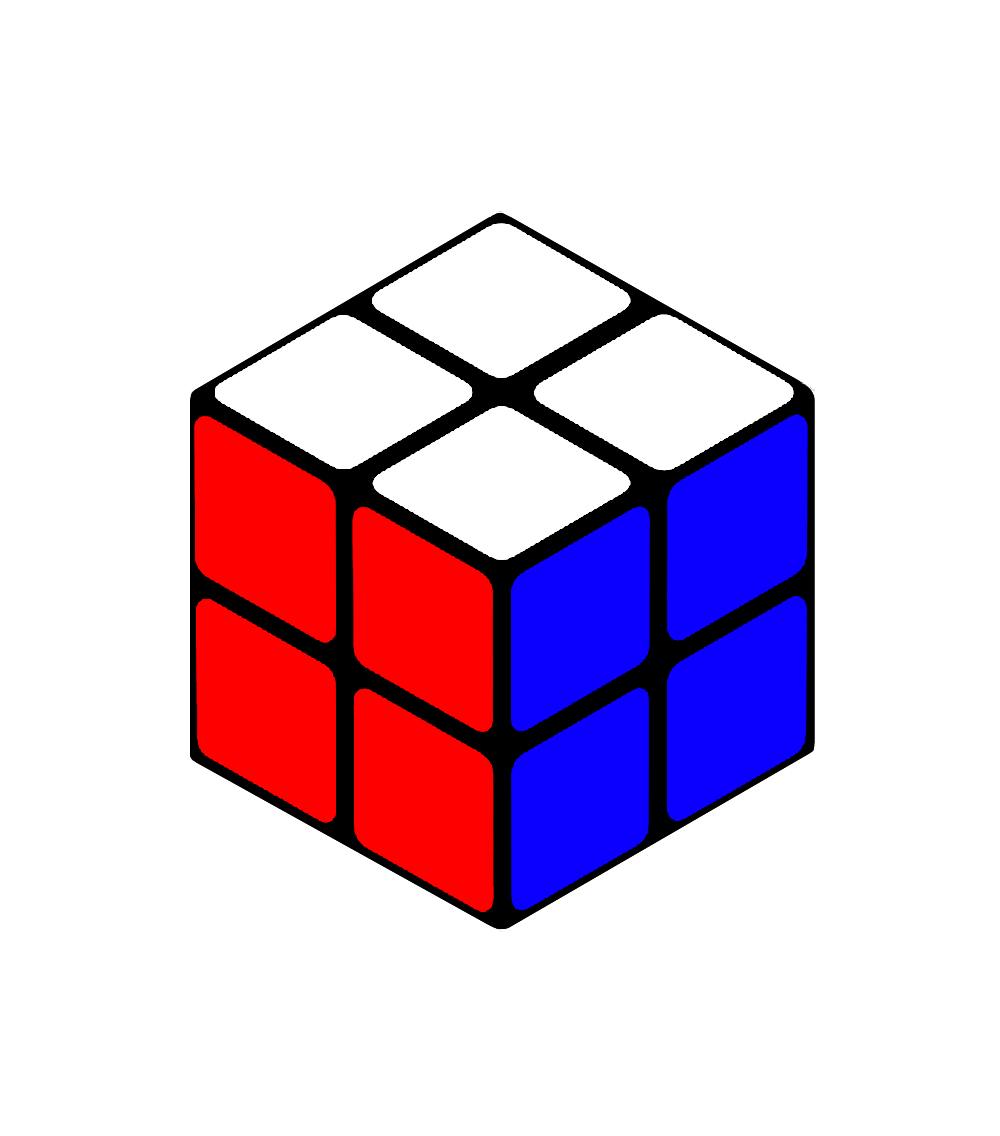
\includegraphics[scale=0.1]{2x2solved.png}
\caption{2x2x2 Zauberwürfel \\ (links in ungelöstem und rechts in gelöstem Zustand (Startkonfiguration)) \\
Der Zauberwürfel wird hier auch Würfel oder Cube genannt.}
\end{figure}
\ \\
Bei der Startkonfiguration (auch Grundposition, Grundstellung) des 2x2x2 Würfels hat jede Seite 4 Farbflächen einer Farbe. Der Würfel ist dann gelöst. \\

\begin{figure}[h]
\centering
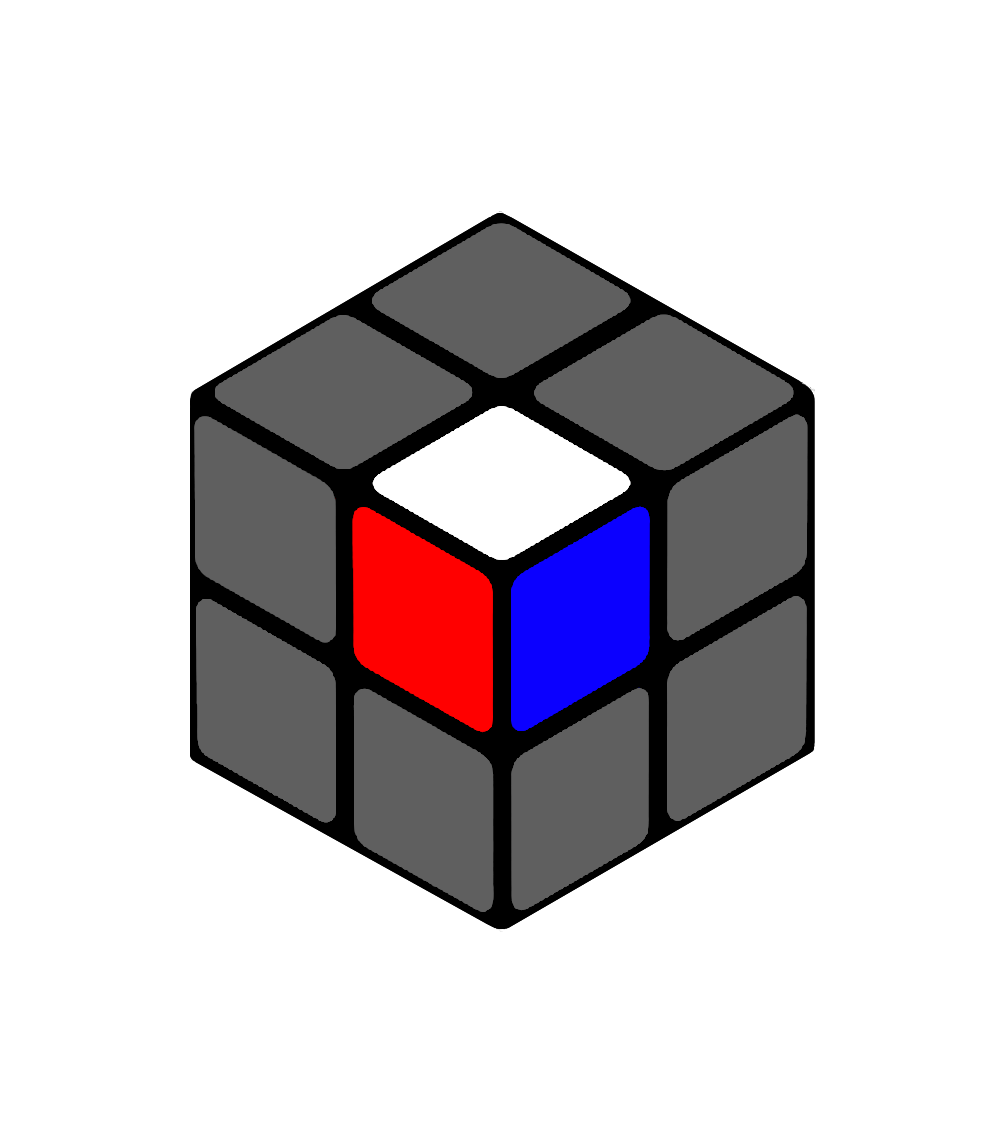
\includegraphics[scale=0.1]{2x2stein.png}
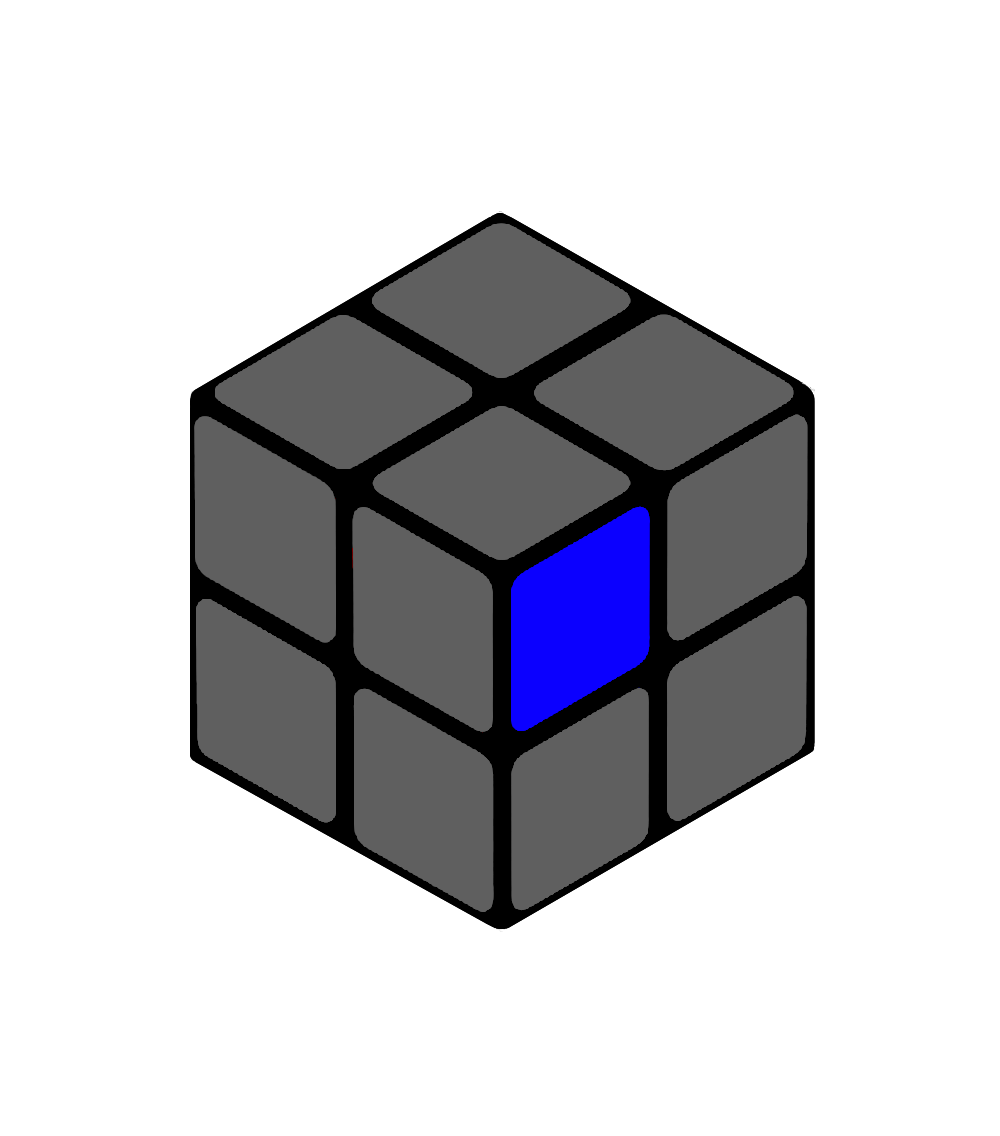
\includegraphics[scale=0.1]{2x2farbflaeche.png}
\caption{Ein 2x2x2 Würfel besteht aus acht (Eck-)Steinen (links), die jeweils drei Farbflächen (rechts) haben. Ein 2x2x2 Zauberwürfel hat also 24 Farbflächen.}
\end{figure} 
$\ $ \\
Die Ecksteine können sich in jeder Ecke befinden, also gibt es pro Eckstein 8 mögliche Positionen im Würfel. Da es 8 Ecksteine gibt, gibt es also $8! = 1 \cdot 2 \cdot 3 \cdot 4 \cdot 5 \cdot 6 \cdot 7 \cdot 8 = 40\, 320$ mögliche Positionen für die Ecksteine. \\
Außerdem können die Ecksteine gedreht sein, also verschiedene Farbflächen oben sein. Da die Steine aus 3 Farbflächen bestehen, können sie durch Rotationen theoretisch 3 verschiedene Ausrichtungen annehmen. Es gibt also $3^8$ Wege, wie die Ecksteine ausgerichtet sein können. \\
Somit ergibt es $3^8 \cdot 8!$ theoretisch mögliche Positionen für den Würfel. Das sind $264\, 539\, 520$ Positionen.\\
Es sind aber nicht alle dieser Positionen valide. Eine Position ist valide, wenn sie durch drehen der Seiten erreicht werden kann, von der Startkonfiguration ausgehend. \\

\begin{figure}[h]
\centering
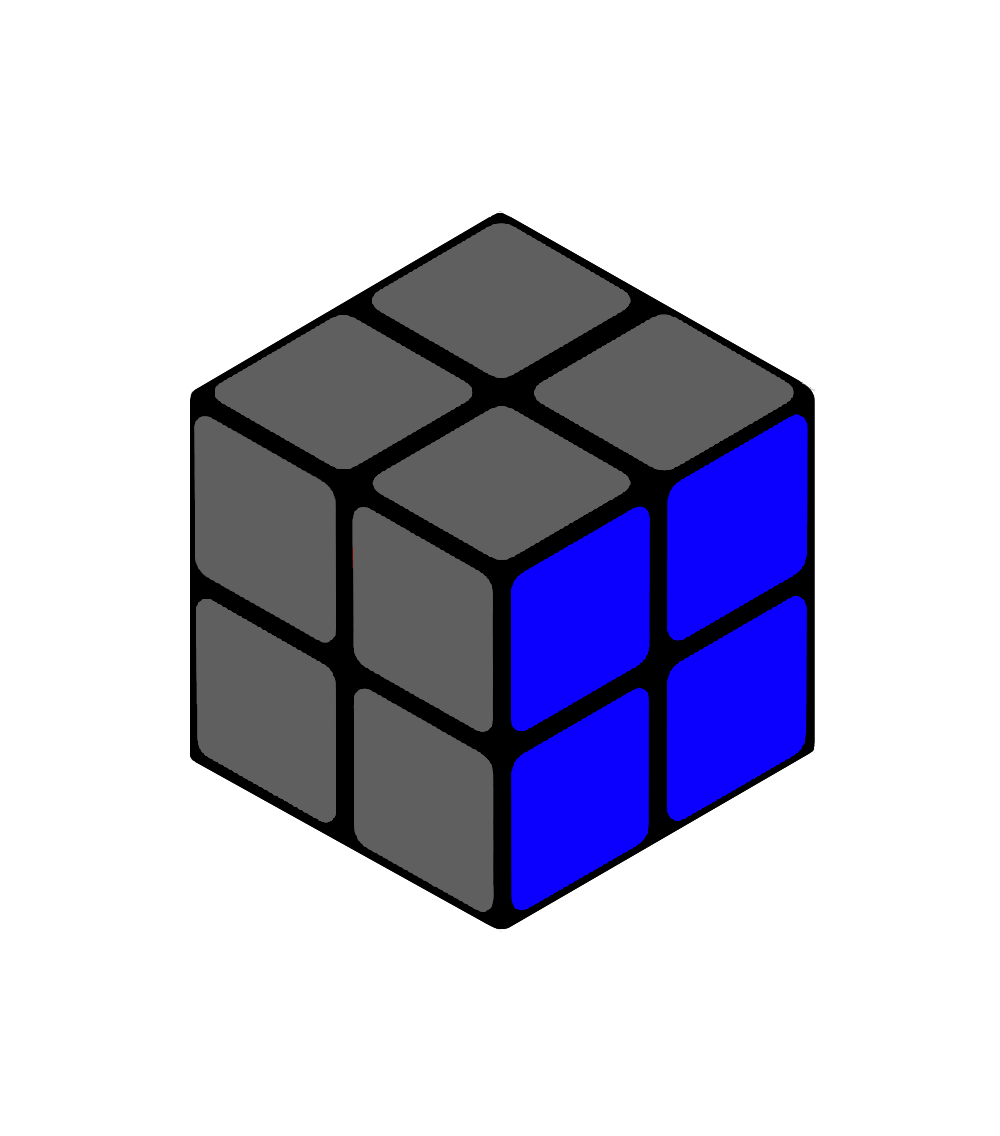
\includegraphics[scale=0.1]{2x2seite.png}
\caption{Der 2x2x2 und der 3x3x3 Zauberwürfel haben jeweils 6 Seiten.}
\end{figure}


\begin{figure}[h]
\centering
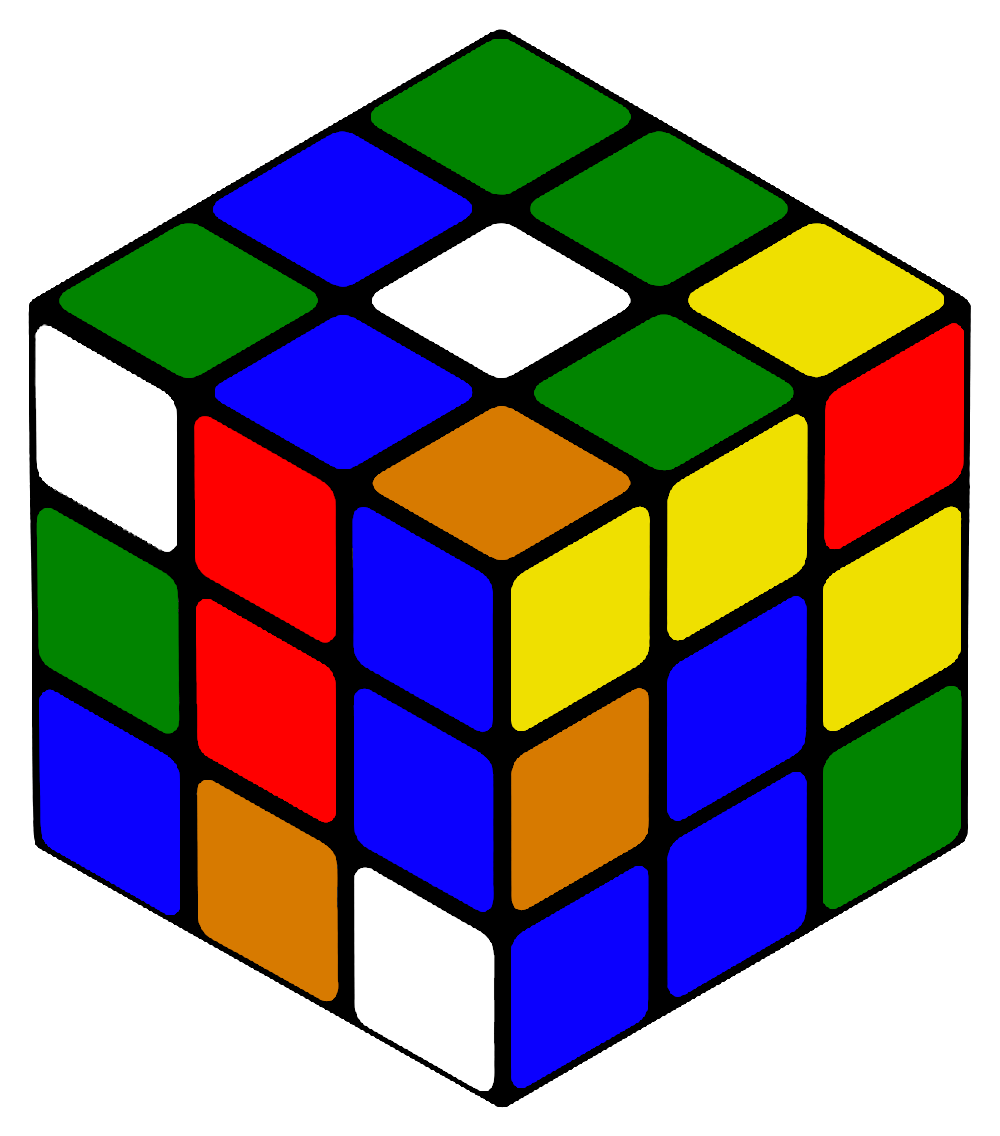
\includegraphics[scale=0.09]{3x3scrambled.png}
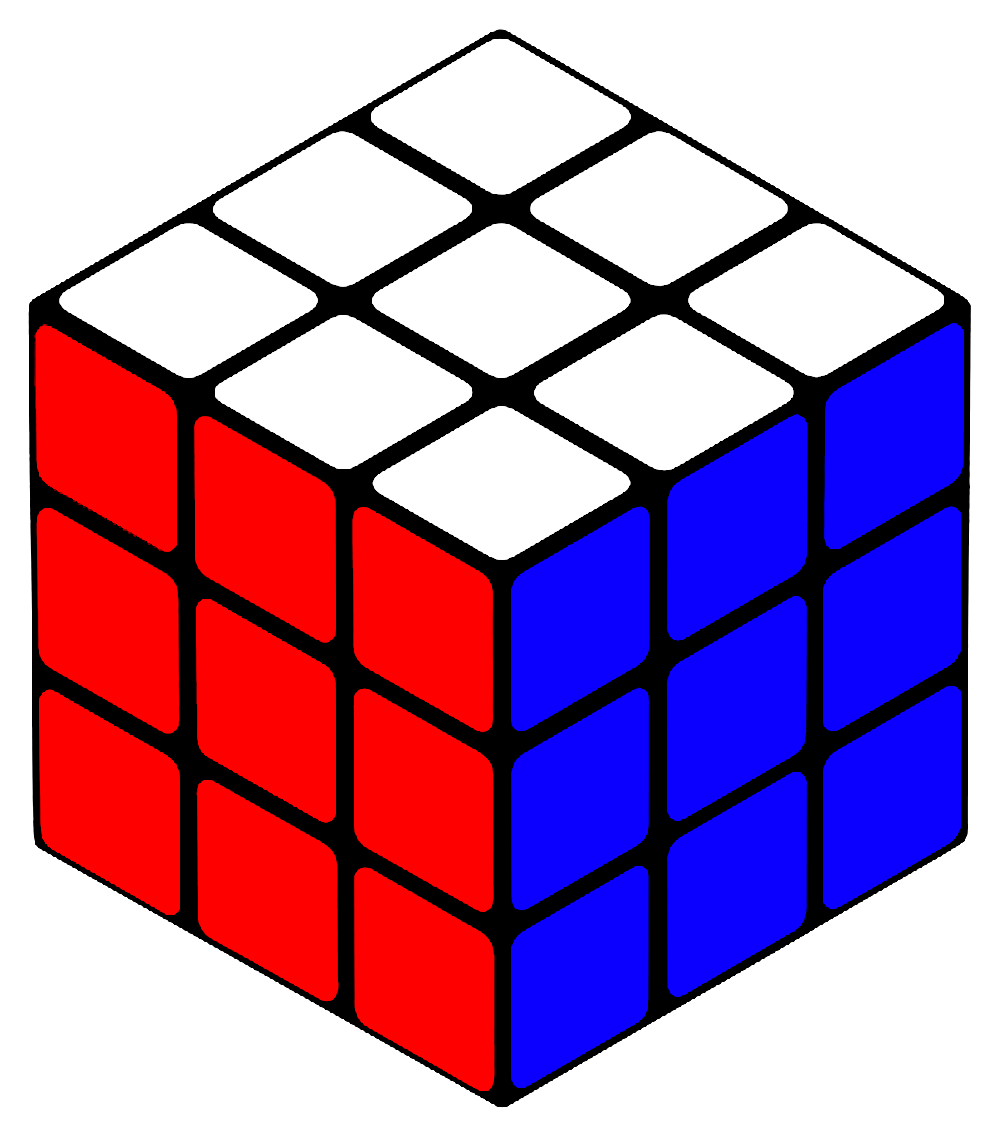
\includegraphics[scale=0.09]{3x3solved.png}
\caption{3x3x3 Zauberwürfel \\ (links in ungelöstem und rechts in gelöstem Zustand (auch Grundstellung))}
\end{figure}

$\ $\\
Im Gegensatz zum 3x3x3 Würfel hat der 2x2x2 Würfel weder Mittelsteine, noch Kantsteine. \\
Das besondere an den Mittelsteinen des 3x3x3 Würfels ist, dass sie bei der Rotation der Seiten (also bei Zügen des Würfels) nicht verändert werden. Somit ist beim 3x3x3 Würfel die obere Seite immer fest zu stellen: Die obere Seite hat immer das weiße Mittelstück in der Mitte. \\
Beim 2x2x2 muss auch noch geprüft werden, ob die aktuelle Konfiguration nicht einer vermeintlich anderen Konfiguration entspricht, bei der nur eine andere Seite nach oben gehalten wird. \\
Die Rotation des gesamten Würfels ist bei dem 3x3x3 Würfel also eindeutig vorgegeben, während sie beim 2x2x2 Würfel gedreht werden kann. \\
\\











%=======================================================================================================







\newpage

\subsection*{Grundzüge des Würfels} \addcontentsline{toc}{subsection}{\protect\numberline{}Grundzüge des Würfels}
Am 2x2x2 Zauberwürfel gibt es sechs verschiedene Drehseiten: oben, unten, links, rechts, vorne und hinten. 
%Da der Würfel aber nur aus zwei Ebenen besteht, entspricht eine Drehung der oberen Ebene nach rechts, einer Drehung der unteren Ebene nach links. \\
%Obwohl ich aber davon ausgehe, den kompletten Würfel beliebig zu rotieren, definiere ich die Drehungen der Ebenen für jede Ebene, damit die Algorithmen anschaulicher sind. Sonst entspräche ja eine Drehung der oberen Ebene im Uhrzeigersinn ($U$) einer dreifachen Drehung der unteren Ebene im Uhrziegersinn ($DDD$) mit anschließender Rotation des kompletten Würfels im Uhrzeigersinn. Es ist aber übersichtlicher, jede Ebenendrehung als einzelnen Zug darzustellen. \\
\begin{figure}[h]
\centering
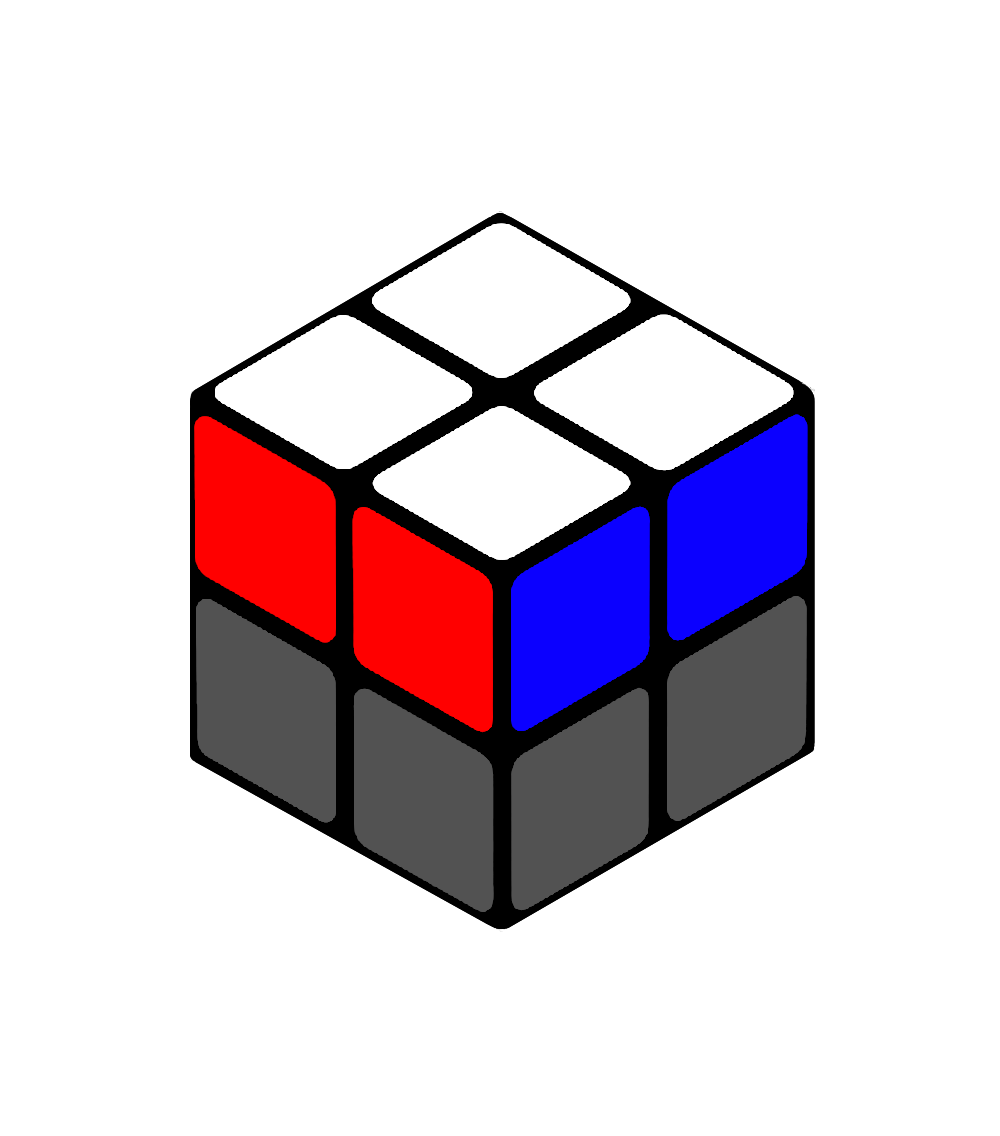
\includegraphics[scale=0.1]{ebene.png}
\caption{Der Würfel hat sechs verschiedene Ebenen. Hier sieht man die obere Ebene farblich markiert.}
\end{figure}

\begin{tabular}{|c|l|}
\hline
Abkürzung & Beschreibung des Zugs \\
\hline
\hline
$U$ & Drehung der oberen Ebene im Uhrzeigersinn \\
\hline
$D$ & Drehung der unteren Ebene im Uhrzeigersinn \\
\hline
$R$ & Drehung der rechten Ebene im Uhrzeigersinn \\
\hline
$L$ & Drehung der linken Ebene im Uhrzeigersinn \\%
\hline
$F$ & Drehung der vorderen Ebene im Uhrzeigersinn \\
\hline
$B$ & Drehung der hinteren Ebene im Uhrzeigersinn \\
\hline
\end{tabular} \\
\\
Die Kürzel stehen für \textit{Up, Down, Right, Left, Front, Back}.  \\
\\
Die entsprechende Ebene wird im Uhrzeigersinn gedreht, wenn man auf diese Ebene schaut. Es wirkt also so, also würde man die untere Ebene gegen den Uhrzeigersinn drehen, wenn man von oben auf den Würfel schaut.  \\
\\
Auf die Rotationsmöglichkeiten des kompletten Würfels gehe ich im Verlauf dieser Arbeit noch ein.
\newpage










%=======================================================================================================









\section{Würfel als Gruppe}

\subsection*{Darstellung des 2x2x2 Zauberwüfels mit dem mathematischen Konstrukt der Gruppe} \addcontentsline{toc}{subsection}{\protect\numberline{}Darstellung des 2x2x2 Wüfels mit dem Konstrukt der Gruppe}

Die Definition einer Gruppe $(G, \circ)$ ist Grundlage für den folgenden Abschnitt:
\begin{itemize}
\item Abgeschlossenheit: $\forall a,b \in G.(a \circ b) \in G $
\item Assoziativität: $\forall a,b,c \in G.(a \circ b) \circ c = a \circ (b \circ c)$
\item Existenz eines neutralen Elements $n$: $\forall a \in G, \exists n \in G.n \circ a = a \circ n = a$ 
\item Existenz eines inversen Elements $a^{-1}$: $\forall a \in G, \exists a^{-1} \in G. a \circ a^{-1} = a^{-1} \circ a = n$ 
\end{itemize}
\ \\
Im folgenden setze ich die Definition der Gruppe des 3x3x3 Würfels aus dem Paper \glqq Group Theory and the Rubik's Cube\grqq \  von Janet Chen \cite{JC} als Gruppe des 2x2x2 Würfels um. Die Gruppe von Janet Chen bezeichne ich als $(G_{3x3x3}, \circ)$, auch wenn er sie als $(G, *)$ bezeichnet hat. Den Namen der Gruppe ändere ich aber, um klar zwischen dem 2x2x2 und dem 3x3x3 Würfel zu differenzieren. Das Symbol des Operators verändere ich, um Verwechslungen mit dem Multiplikationsoperator zu vermeiden. \\
\\ 
Die Gruppe des 2x2x2 Würfels nenne ich $(G_{2x2x2}, \circ)$. \\
\\
Die Menge $G_{2x2x2}$ besteht aus allen möglichen Zügen des Würfels. Beispielsweise die Drehung der oberen Ebene ist ein Zug. Ein Zug kann aber auch aus mehreren Drehungen bestehen, z.B. das Drehen der oberen Ebene, gefolgt von dem Drehen der rechten Ebene stellt ebenfalls einen Zug dar. \\
Wenn zwei Züge die gleiche Würfelposition hervorrufen, sind die beiden Züge "gleich". Beispielsweise eine Drehung um $180^{\circ}$ nach links oder nach rechts von einer Ebene führt zu dem gleihen Ergebnis und somit werden diese beiden Züge als gleich angesehen. \\
\\
Der Operator $\circ$ ist als Konkatenation zweier Züge definiert. Wenn $Z_1 \in G_{2x2x2}$ und $Z_2 \in G_{2x2x2}$ zwei Züge sind, dann bedeutet $Z_1 \circ Z_2$, dass zuerst $Z_1$ und dann $Z_2$ ausgeführt wird. (Außerdem gilt dann auch $Z_1 \circ Z_2 \in G_{2x2x2}$.) \\
Im folgenden werde ich begründen, wieso $(G_{2x2x2}, \circ)$ eine Gruppe ist, indem ich $(G_{2x2x2}, \circ)$ bezüglich der Gruppenkriterien untersuche: \\
\begin{itemize}
\item Abgeschlossenheit: \\ 
$\forall Z_1,Z_2 \in G_{2x2x2} .  (Z_1 \circ Z_2) \in G_{2x2x2} $ \\
\\
Die Gruppe $G_{2x2x2}$ ist abgeschlossen unter dem Operator $\circ$. Wenn $Z_1 $ und $Z_2$ Züge sind und somit Elemente von $G_{2x2x2}$, dann ist auch $Z_1 \circ Z_2$ ein Element der Gruppe, da alle Züge in $G_{2x2x2}$ enthalten sind. 

\item Assoziativität:\\ 
$\forall Z_1,Z_2,Z_3 \in G_{2x2x2}.(Z_1 \circ Z_2) \circ Z_3 = Z_1 \circ (Z_2 \circ Z_3)$ \\
\\
Die Züge $Z_i \in G_{2x2x2}$ können gruppiert werden und somit gilt die Assoziativität. \\
Um die Assoziativität zu zeigen, werde ich eine Schreibweise für das Ausführen der Züge einführen. Ich nenne einen bestimmten Stein im Würfel nun $s$. Beim Ausführen eines Zuges $Z$ schreibe ich nun $Z(s)$, um die neue Position des Steines zu erhalten. Die Positionen sind (wie oben beschrieben) 3-Buchstaben-Kürzel, bestehend aus $u, d, l, r, t, b$. \\
Wenn wir nun $Z_1 \circ Z_2 $ haben, wird zuerst $Z_1$ und dann $Z_2$ ausgeführt. $Z_1(s)$ bewegt den Stein s zu der Position $Z_1(s)$. Der Zug $Z_2$ bewegt den Stein dann zu der Position $Z_2(Z_1(s))$. Also gilt $Z_1 \circ Z_2 = Z_2(Z_1(s))$. \\
\\
Nun muss noch $(Z_1 \circ Z_2) \circ Z_3 = Z_1 \circ (Z_2 \circ Z_3)$ gezeigt werden. Ich zeige also, dass sich $(Z_1 \circ Z_2) \circ Z_3$ und $Z_1 \circ (Z_2 \circ Z_3)$ beide zu $Z_3(Z_2(Z_1(s))$ umformen lassen: \\
\begin{align*}
& (Z_1 \circ Z_2) \circ Z_3  \\
\Rightarrow (&(Z_1 \circ Z_2) \circ Z_3)(s) \\
= & Z_3(Z_1 \circ Z_2)(s)) \\
= & Z_3(Z_2(Z_1(s)))  
\end{align*}
\begin{align*}
&Z_1 \circ (Z_2 \circ Z_3) \\
\Rightarrow (&Z_1 \circ (Z_2 \circ Z_3))(s) \\
= (&Z_2 \circ Z_3)(Z_1(s)) \\
= \ \ & Z_3(Z_2(Z_1(s)))  
\end{align*}
Somit ist $(G_{2x2x2}, \circ)$ assoziativ.

\item Existenz eines neutralen Elements $N$:  \\
$\forall Z_1 \in G_{2x2x2}, \exists N \in G_{2x2x2}.N \circ Z_1 = Z_1 \circ N = Z_1$ \\
\\
Das neutrale Element $N$ muss aus der Menge $G_{2x2x2}$ der Züge sein und es muss gelten: $N \circ Z_1 = Z_1 \circ N = Z_1$. Somit ist das neutrale Element der Gruppe $(G_{2x2x2}, \circ)$ der \glqq leere \grqq \ Zug. Es werden also keine der Ebenen des Würfels gedreht. Wenn man also einen Zug $Z$ ausführt und dann den Zug $N$, bedeutet das so viel wie \glqq erst $Z$ ausführen und dann nichts \grqq , was das gleiche ist wie $Z$ auszuführen.


\item Existenz eines inversen Elements $Z_1^\prime$: \\ 
$\forall \  Z_1 \in G_{2x2x2},\ \exists \  Z_1^\prime \in G_{2x2x2}.  \ \ Z_1 \circ Z_1^\prime = Z_1^\prime \circ Z_1 = N$  \\
\\
Da $Z$ ein Zug ist, kann man diesen auch rückgängig machen. Man muss die einzelnen Ebenenrotationen nur rückwärts und von hinten durchführen, um den Zug zu invertieren. Dann gilt $Z_1 \circ Z_1^\prime = Z_1^\prime \circ Z_1 = N$.
\end{itemize}
Somit ist $(G_{2x2x2}, \circ)$ eine Gruppe. \\ 
\\
Damit $(G_{2x2x2}, \circ)$ eine kommutaive Gruppe (oder Abelsche Gruppe) ist, muss zusätzlich noch die Kommutativität gelten. \\
Dies ist nicht der Fall, da beispielsweise eine Rotation der rechten Ebene im Uhrzeigersinn ($R$) und eine Rotation der vorderen Ebene im Uhrzeigersinn ($F$) in umgekehrter Reihenfolge ein anderes Ergebnis haben. Das sieht grafisch dargestellt so aus: \\
\begin{figure}[h]
\centering
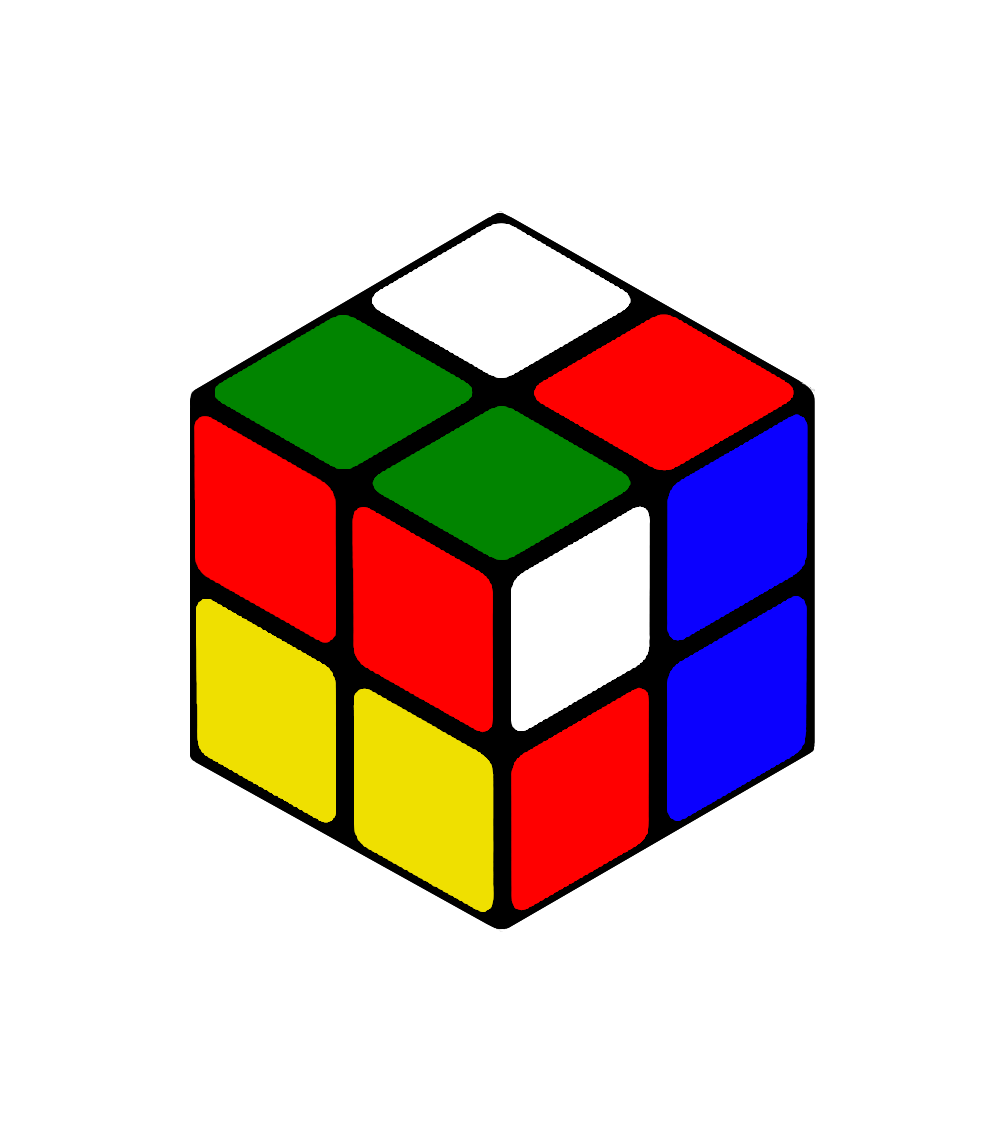
\includegraphics[scale=0.1]{RF.png}
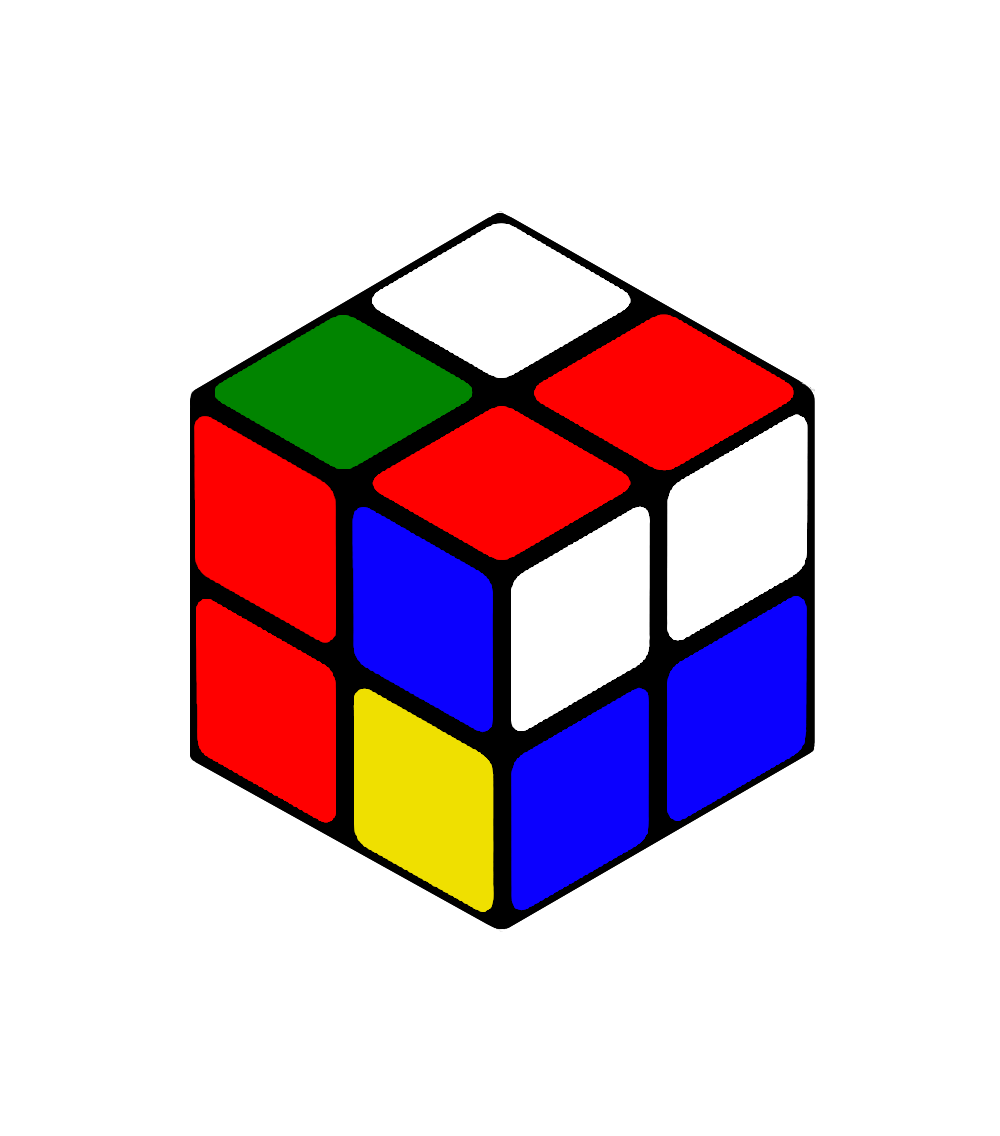
\includegraphics[scale=0.1]{FR.png}
\caption{links: Würfel nach Zug $RF$, rechts: Würfel nach Zug $FR$, \\ ausgehend von Startkonfiguration}
\end{figure} \ \\
Außerdem wäre das Lösen des Würfels trivial, wenn die Kommutativität gelten würde.\cite{TD} \\
Es gilt also nicht $\forall \  Z_1, Z_2 \in G_{2x2x2}. Z_1 \circ Z_2 = Z_2 \circ Z_1$. Der $\circ$-Operator der Gruppe ist also nicht kommutativ. \\
\\
\\
Das mehrfache Ausführen der Züge ($U, D, F, B, L, R$) stelle ich mit Exponenten dar. So schreibe ich beispielsweise für $RR$ (also zwei mal eine Drehung der rechten Ebene im Uhrzeigersinn) auch als $R^2$. \\
Wenn man eine Ebene vier mal dreht, ist der Würfel wieder in der vorherigen Position. Somit gilt also beispielsweise $RRRR=R^4=N$, wobei $N$ für das neutrale Element (also den leeren Zug) steht. Das gilt für alle Züge des Würfels:
\\
\begin{align*}
RRRR & =R^4 =N \\
LLLL & =L^4 =N \\
UUUU & =U^4 =N \\
DDDD & =D^4 =N \\
FFFF & =F^4 =N \\
BBBB & =B^4 =N \\
\end{align*}
Somit gilt dann auch $Z^0=N$, mit $Z$ als beliebigen Zug und $N$ als neutrales Element. \\
In der mathematischen Schreibweise sieht das so aus: $\forall Z \in G_{2x2x2} \ . \ Z^0=N$. \\
Es gilt also für alle Züge $Z \in G_{2x2x2}$: 
\begin{align*}
Z^0 & =N \\
Z & =Z^1 \\
ZZ & =Z^2 \\
ZZZ & =Z^3 \\
\end{align*}
Für \glqq einelementige Züge\grqq \  (also $U, D, F, B, L$ oder $R$) gilt auch $YYYY =Y^4=N=Y^0$.
Man kann den Exponenten in diesem Fall also $modulo \ 4$ rechnen, da vier Drehungen einer Ebene nacheinander wieder zum Startzustand führen. \\
Es gilt dann also: \\
$\forall \  Y \in \{U, D, F, B, L, R\}, n \in \mathbb{N} \ . \ Y^n=Y^{n \mod 4}$.
\newpage








%=======================================================================================================









\section{Konfiguration des Würfels}
Die Konfiguration des Würfels, also die Position/Verdrehung des Würfels setzt sich aus zwei Parametern zusammen: 
\begin{itemize}
\item Position der Ecksteine (angegeben als $\sigma$)
\item Ausrichtung der Ecksteine (angegeben als $x_i$)
\end{itemize}
Also kann die Konfiguration des Würfels als ein 2-Tupel geschrieben werden: $(\sigma, x)$. \\
\\
Der Würfel kann aber auch komplett gedreht werden, ohne Züge auszuführen.









%=======================================================================================================










\subsection*{Positionen der Steine im Würfel} \addcontentsline{toc}{subsection}{\protect\numberline{}Positionen der Steine im Würfel}

Um die Übergänge der Würfelsteine als Funktion darzustellen, definiere ich eine bijektive Funktion $\sigma$ für jede Ebenenrotation. $\sigma$ bildet jede der Würfelpositionen auf die neue Position ab. \\
\\
Die Würfelpositionen habe ich wie folgt eingeteilt: \\
\begin{figure}[H]
\centering
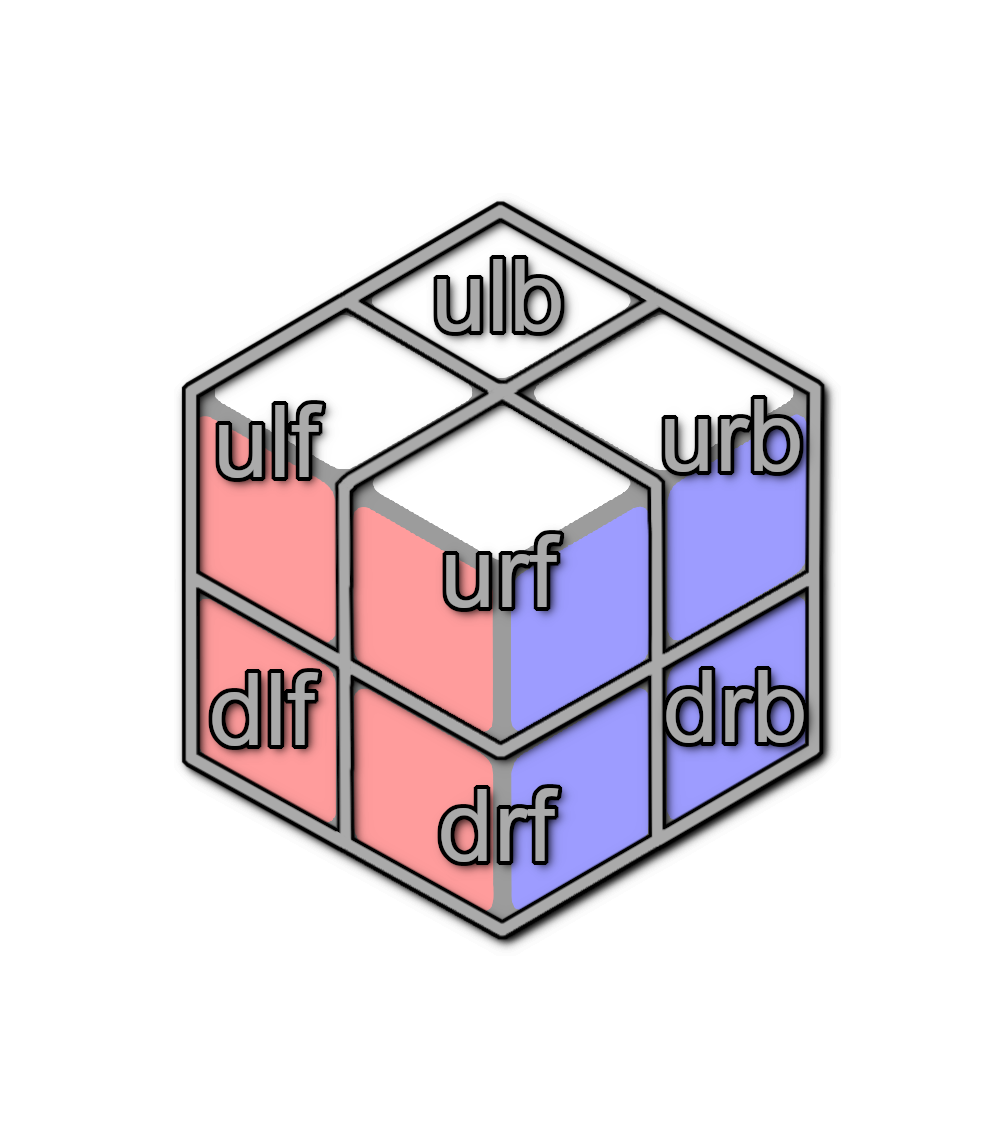
\includegraphics[scale=0.15]{caged_positions.png} \\
\caption{Die einzelnen Steinpositionen werden mit den Kürzeln benannt, die \textit{up, down, left, right, front und back} beschreiben.}
\end{figure}

\begin{figure}[H]
\centering
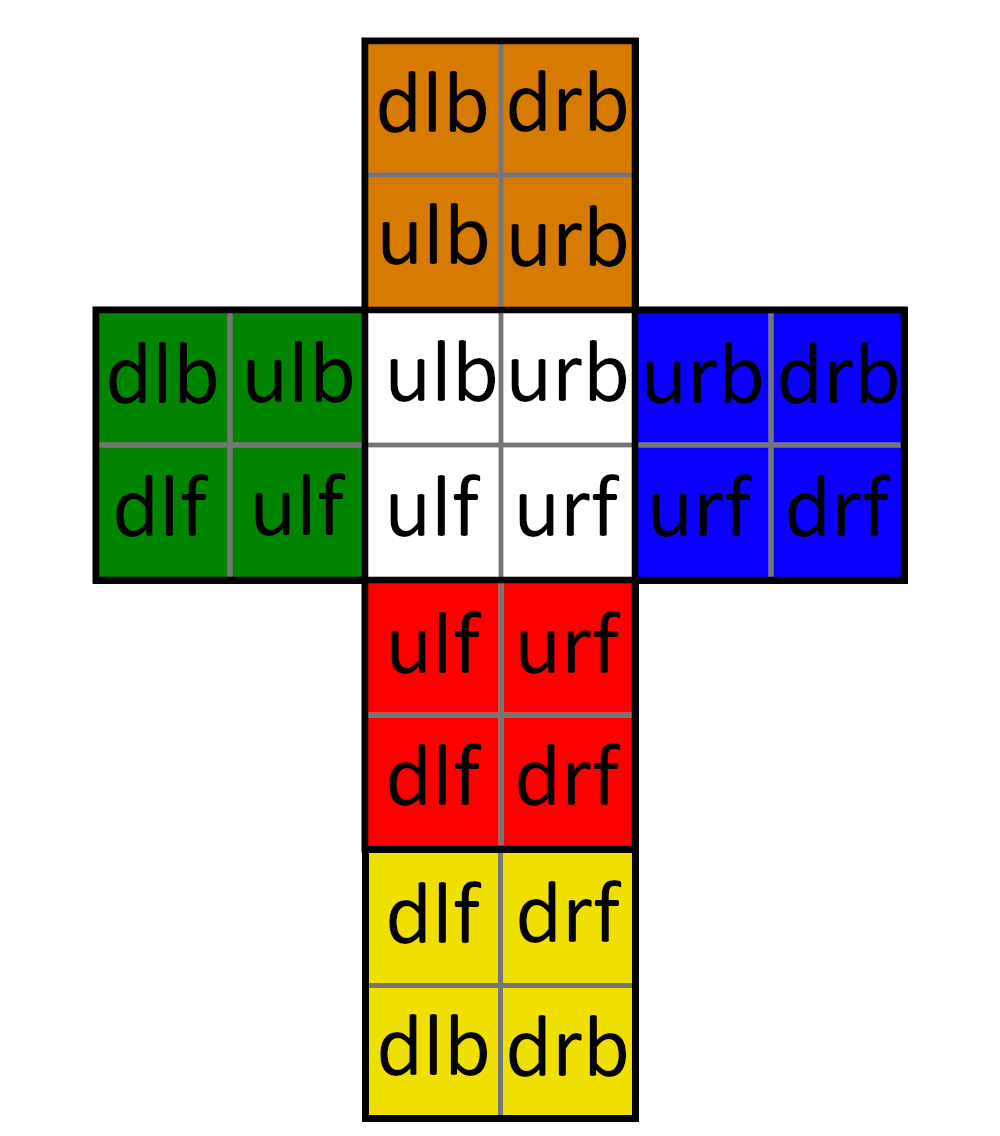
\includegraphics[scale=0.15]{foldedout_cage.png}
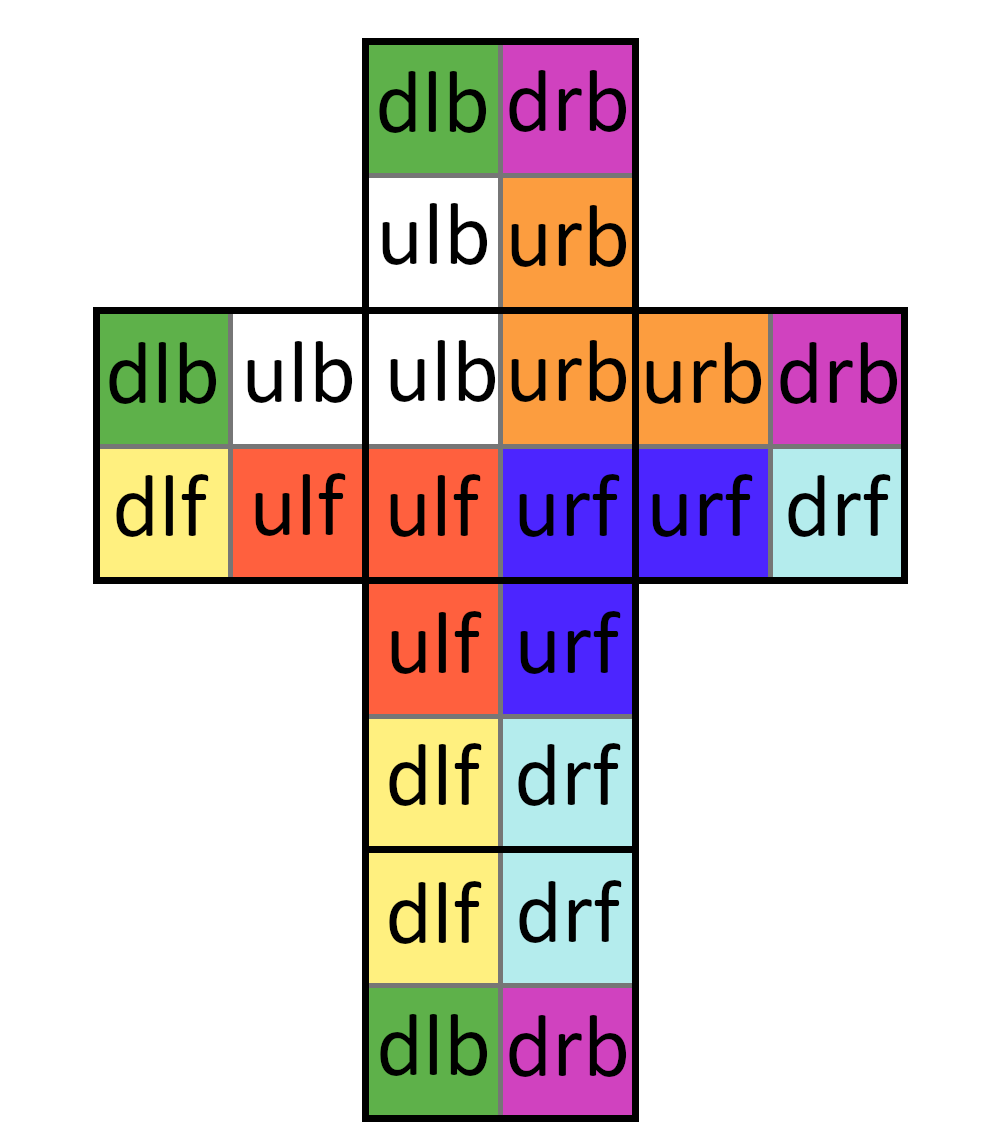
\includegraphics[scale=0.15]{foldedout_cage_color.png}
\end{figure}
\ \\
\\
Ich ordne jeder Steinposition einen einzigartigen Namen zu, um mich darauf zu beziehen. Dabei gehe ich davon aus, dass die weiße Seite in der Startkonfiguration oben ist. Die Steinposition beschreibe ich mich 3 Buchstaben, die aus den Kürzeln \textit{u, d, l, r, f, b} bestehen. Diese Kürzel stehen für \textit{up, down, left, right, front, back}. \\
Somit heißt die Steinposition oben links also $ulf$ (für up, left und front). 
\\
\\
Jeder Stein bekommt auch einen einzigartigen Namen, der seiner Steinposition im gelösten Zustand entspricht. Beispielsweise liegt der Stein $ulf$ im gelösten Zustand an der Steinposition $ulf$.
\\ 
\\
Nun definiere ich $\sigma_U$ für eine Drehung der oberen Ebene um 90$^\circ$ im Uhrzeigersinn: \\
Ich beschreibe $\sigma_U$ ausführlich und gebe verschiedene Schreibweisen an. Die weiteren Drehungen funktionieren dann analog. \\
\\
Die Drehung der oberen Ebene sieht grafisch dargestellt so aus: \\
\begin{figure}[H]
\centering
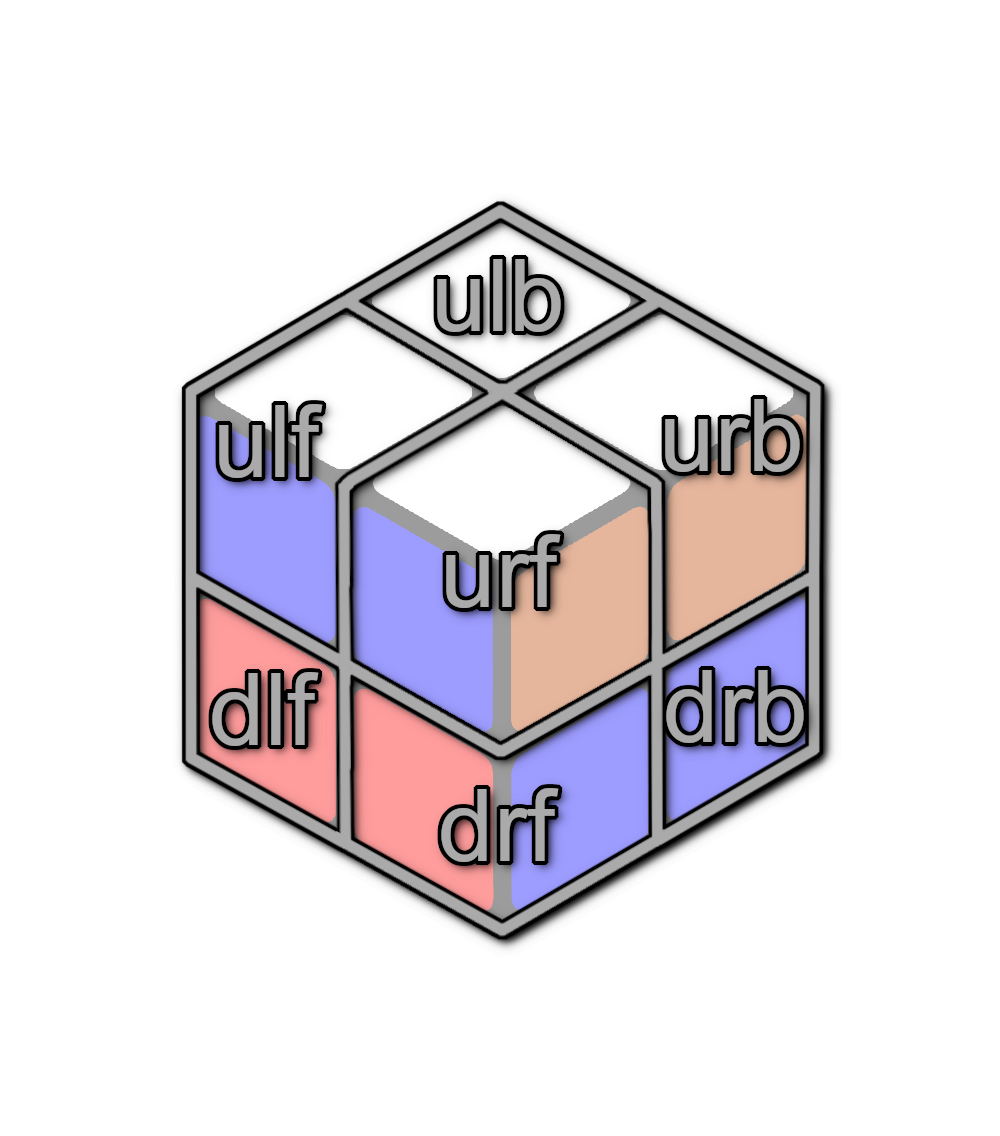
\includegraphics[scale=0.13]{caged_spin.png}
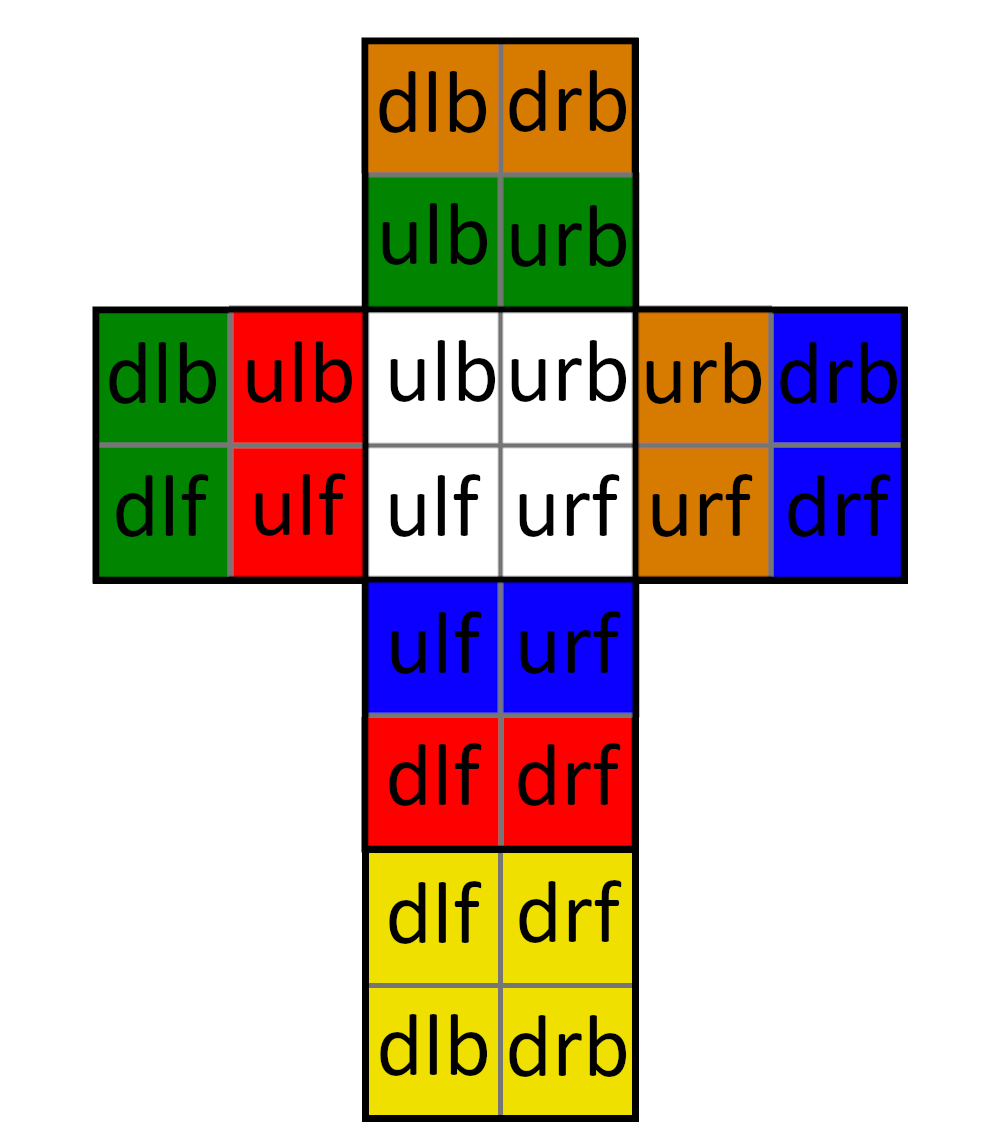
\includegraphics[scale=0.13]{foldedout_spin.png}
\end{figure}
\ \\
$\sigma_U(ulf)=ulb$ \ \ \ \ \ \ \ \ $\sigma_U(ulb)=urb$ \ \ \ \ \ \ \ \ $\sigma_U(urb)=urf$ \ \ \ \ \ \ \ \ $\sigma_U(urf)=ulf$ \\
$\sigma_U(dlf)=dlf$ \ \ \ \ \ \ \ \ $\sigma_U(dlb)=dlb$ \ \ \ \ \ \ \ \ \ $\sigma_U(drb)=drb$ \ \ \ \ \ \ \ \ $\sigma_U(drf)=drf$ \\
\\
Das kann man auch in der Form $i \mapsto j$ schreiben: \\
\\
$ulf \mapsto ulb$ \ \ \ \ \ \ \ \ $ulb \mapsto urb$ \ \ \ \ \ \ \ \ $urb \mapsto urf$ \ \ \ \ \ \ \ \ $urf \mapsto ulf$ \\
$dlf \mapsto dlf$ \ \ \ \ \ \ \ \ $dlb \mapsto dlb$ \ \ \ \ \ \ \ \ \ $drb \mapsto drb$ \ \ \ \ \ \ \ \ $drf \mapsto drf$ \\
\\
Daraus entstehen folgende Zykel: $\sigma_U = \ (ulf \ ulb \ urb \ urf)\ (dlf)\ (dlb)\ (drb)\ (drf)$ \\ \\
Die Zykel mit nur einem Element müssen nicht aufgeschrieben werden. Dann ergibt sich $\sigma_U = \ (ulf \ ulb \ urb \ urf)$, was den Zykel beschreibt, in dem die Steine rotiert werden, wenn die obere Ebene gedreht wird. \\
\\
Die Drehungen der anderen Ebenen können durch folgende Zykel beschrieben werden: \\
\begin{align*}
\sigma_U & =\ (ulf \ ulb \ urb \ urf) \\
\sigma_D & =\ (dlf \ drf \ drb \ dlb) \\
\sigma_F & =\ (ulf \ urf \ drf \ dlf) \\
\sigma_B & =\ (ulb \ dlb \ drb \ urb) \\
\sigma_L & =\ (ulb \ ulf \ dlf \ dlb) \\
\sigma_R & =\ (urb \ drb \ drf \ urf) \\
\end{align*}
Die Identitätspermutation schreibe ich als $\sigma = 1$.










%=======================================================================================================









\subsection*{Ausrichtung der Steine} \addcontentsline{toc}{subsection}{\protect\numberline{}Ausrichtung der Steine}
Der 2x2x2-Würfel besteht aus 8 Ecksteinen, die jeweils 3 Farbflächen haben. Somit hat jeder Stein 3 mögliche Ausrichtungen. \\
Um die Ausrichtung der Steine zu erkennen, bekommen Würfelpositionen an einer Farbfläche einer Nummer zugeordnet. Dafür habe ich die weißen und die gelben Seiten markiert und nummeriert. Auf diese Nummern beziehe ich mich als $x_i \in \lbrace 1, 2, 3, 4, 5, 6, 7, 8 \rbrace$ mit $x_1$ als Position 1, $x_2$ als Position 2, usw.
\begin{figure}[H]
\centering
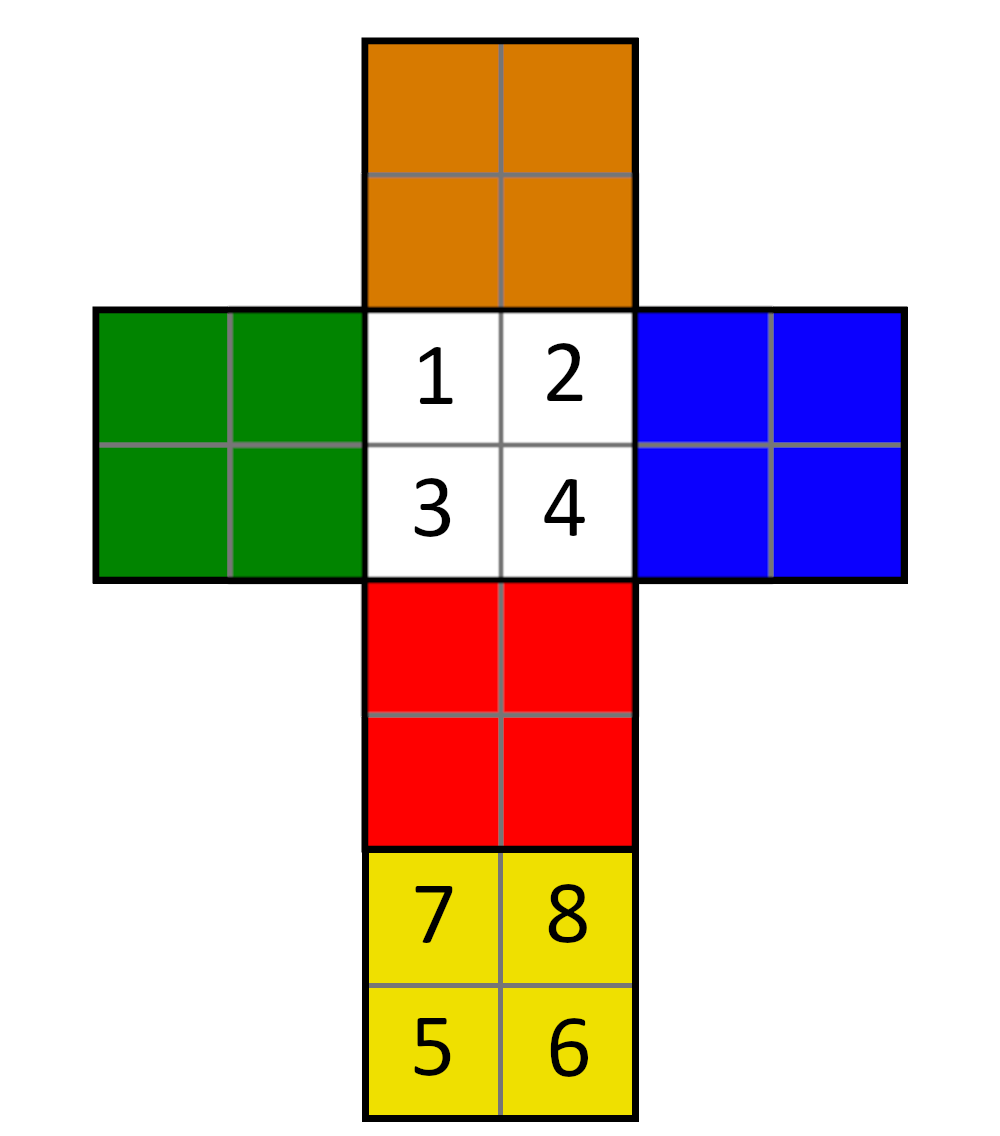
\includegraphics[scale=0.1]{foldedout_numbers.png}
\end{figure}
\ \\
Außerdem bekommt jeder Stein an jeder Farbfläche eine Zahlenzuordnung. Da jeder Stein 3 Ausrichtungen haben kann, nummeriere ich mit 0, 1 und 2. Ich beginne mit der weißen/gelben Fläche bei 0 und zähle dann im Uhrzeigersinn die Flächen. \\
\begin{figure}[H]
\centering
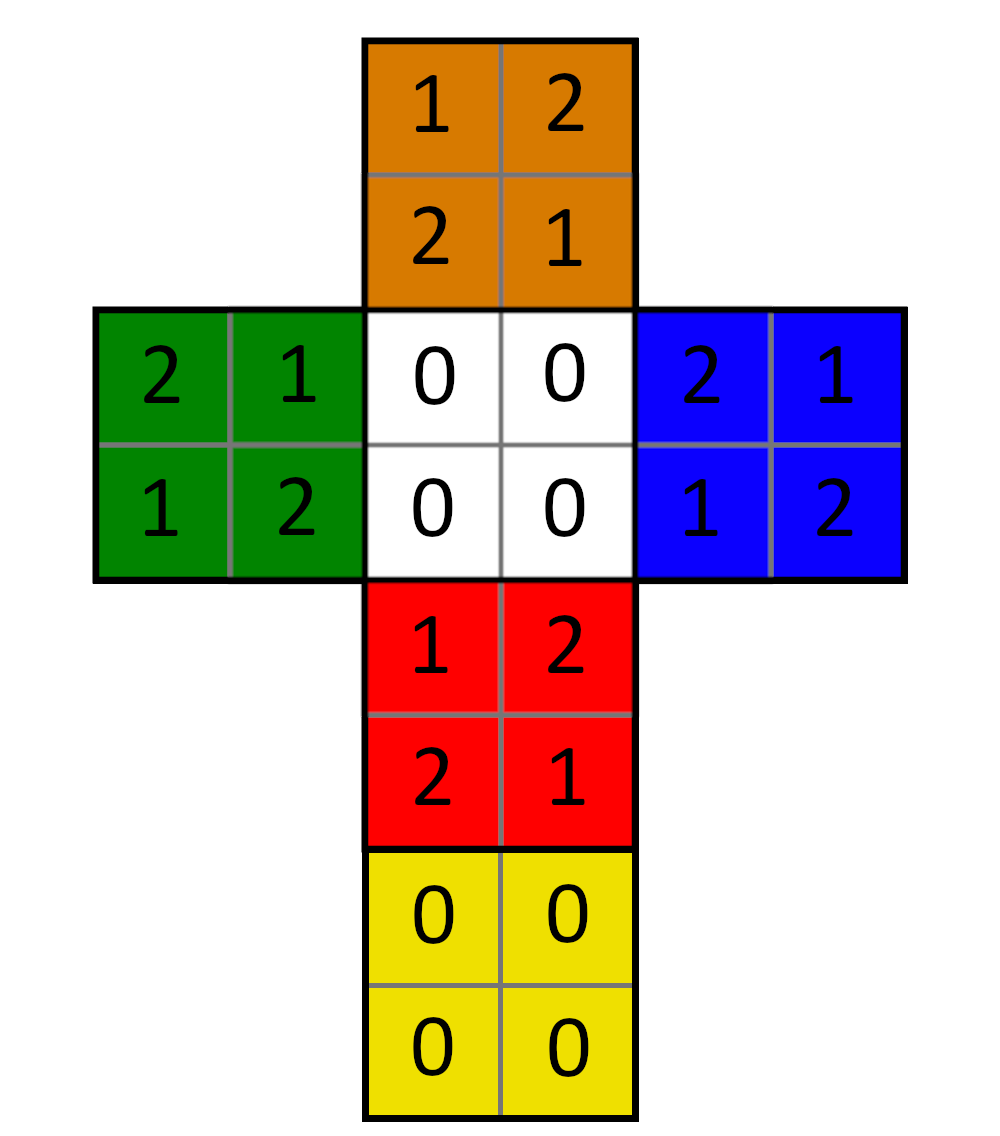
\includegraphics[scale=0.1]{foldedout_012.png}
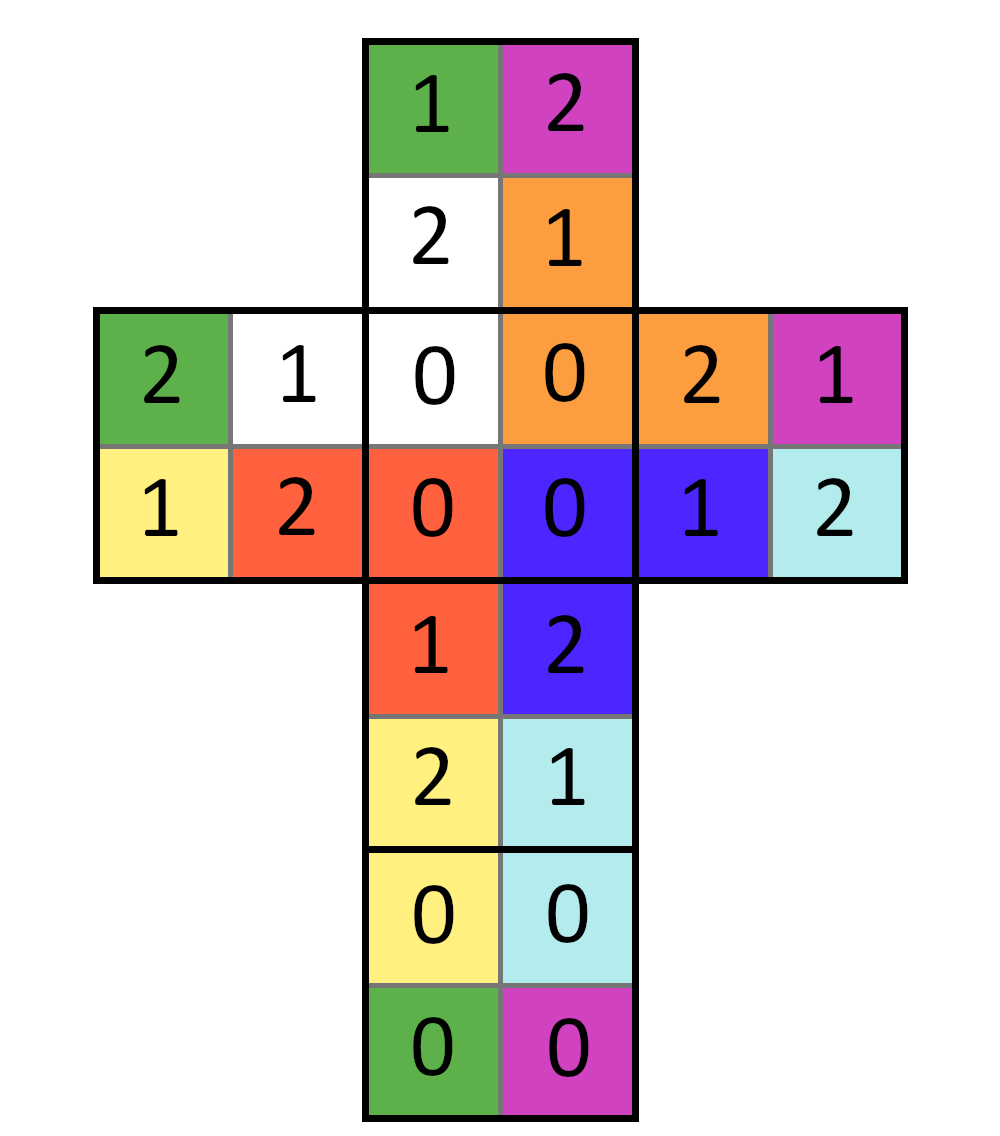
\includegraphics[scale=0.1]{foldedout_c_012.png}
\end{figure}
\ \\
In der Startkonfiguration sind alle $x_i = 0$, also $x=(0, 0, 0, 0, 0, 0, 0, 0)$. Das schreibe ich kurz als $x=0$.\\
\ \\
Nun stelle ich dar, wie sich die Nummerierung der Farbflächen verändert, wenn der Zug $R$ ausgeführt wird. $R$ ist eine Rotation der rechten Ebene um 90$^\circ$ im Uhrzeigersinn. \\
Die Nummerierungen der Position ($x$) bleiben an der gleichen Position, die Nummerierungen ($0, 1, 2$) der Farbflächen ändern sich mit Rotation der Ebene und ermöglichen so eine Zuordnung der Ausrichtung der Ecksteine. \\
Die linke Seite der Würfels wird dabei nicht beeinträchtig, also sind die Flächen an den Positionen $x_1, x_3, x_5, x_7$ alle 0. \\
Die anderen Positionen haben nun aber andere Farbflächen: \\
$x_2 = 2$ \ \ \ \ $x_4 = 1$ \ \ \ \ $x_6 = 1$ \ \ \ \ $x_8 = 2$  \\
Also $x = (0, 2, 0, 1, 0, 1, 0, 2)$ nach dem Zug $R$. \\
\begin{figure}[H]
\centering
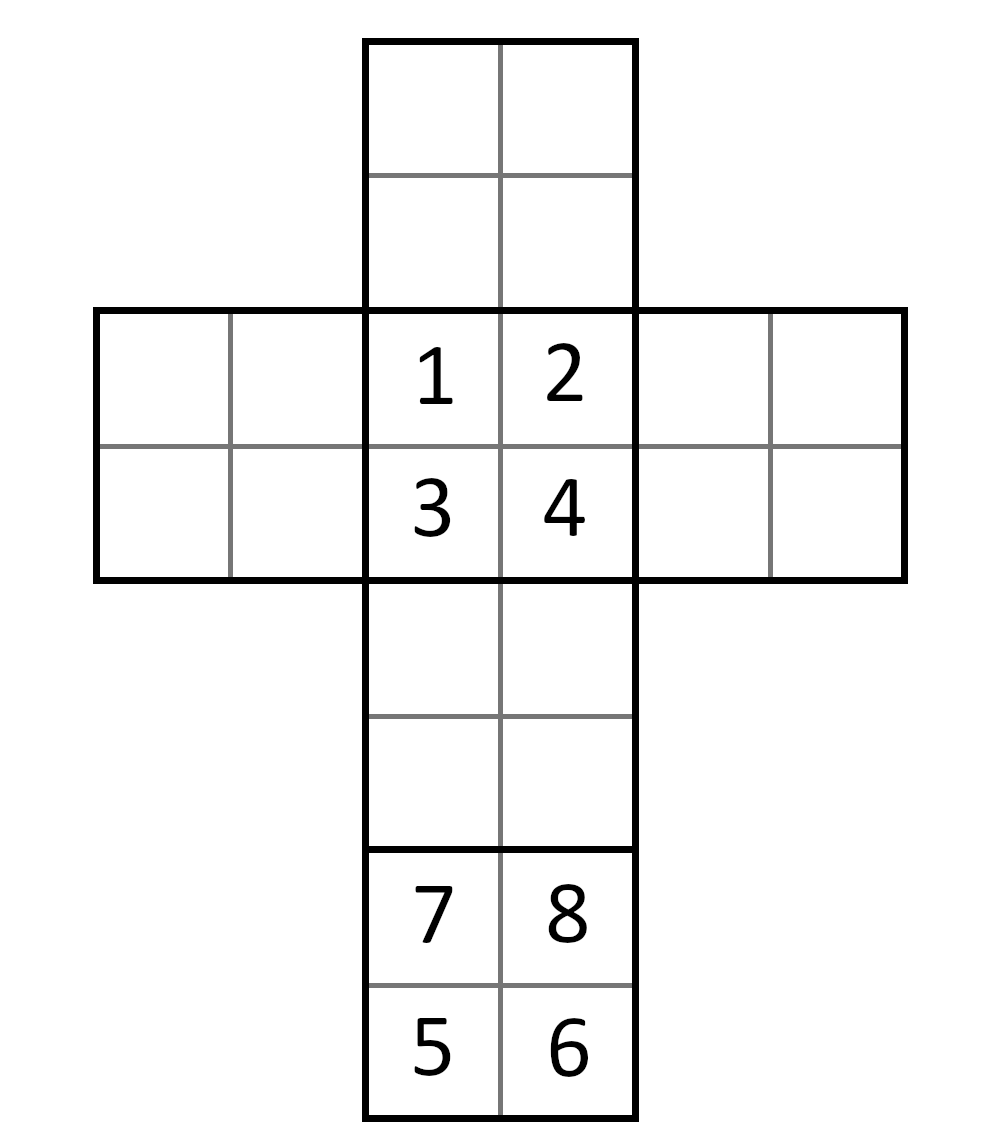
\includegraphics[scale=0.1]{foldedout_012_white.png}
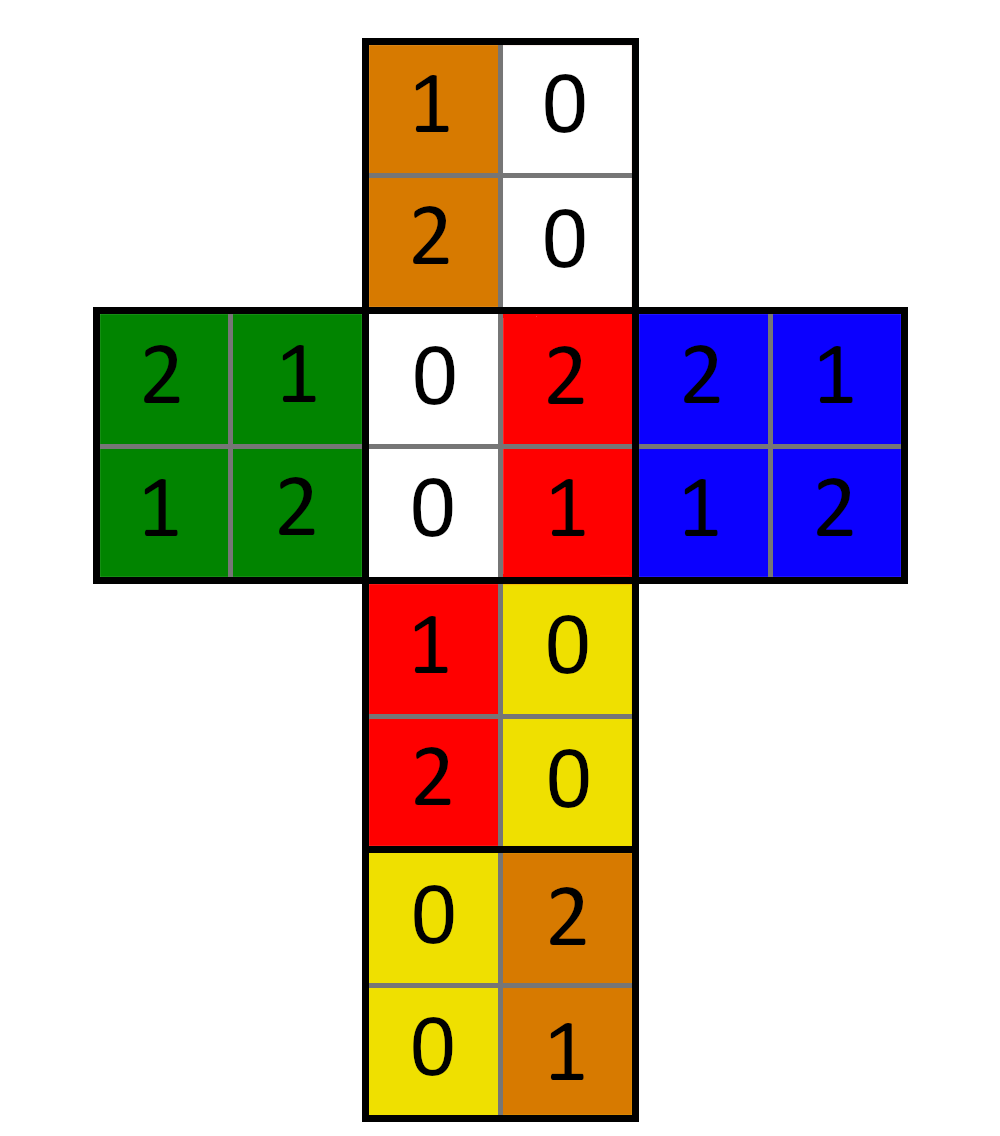
\includegraphics[scale=0.1]{foldedout_012_spin.png}
\caption{links: Positionen $x_1$ bis $x_8$, rechts: Veränderung der nummerierten Ecksteine nach dem Zug $R$}
\end{figure}









%=======================================================================================================












\subsection*{Züge als Gruppenoperation}\addcontentsline{toc}{subsection}{\protect\numberline{}Züge als Gruppenoperation}

Wenn der Zauberwürfel in einer Konfiguration $C=(\sigma, x)$ ist, wird der Würfel durch das Ausführen eines Zuges $M \in G_{2x2x2}$ in eine neue Konfiguration gebracht. Diese Konfiguration schreibe ich als $C \cdot M$. \\
\\
Definition einer Gruppenoperation mit der Gruppe $(G_{2x2x2}, \circ)$ und der Menge $C$:
\begin{itemize}
\item $\cdot: C \times G_{2x2x2} \rightarrow C$ mit $(c, g) \rightarrow c \cdot g $
\item $c \cdot N = x$ für alle $c \in C$ und das neutrale Element $N \in G_{2x2x2}$  
\item $c \cdot (u \circ v) = (c \cdot h) \cdot v$ für alle $u, v \in G_{2x2x2}$ und $c \in C$
\end{itemize}
\ \\
Angenommen der Würfel befindet sich in der Konfiguration $C$. Wenn nun der Zug $M_1 \in G_{2x2x2}$ ausgeführt wird, ist die neue Konfiguration des Würfels $C \cdot M_1$. Wenn nun noch ein weiterer Zug $M_2 \in G_{2x2x2}$ ausgeführt wird,ist die neue Konfiguration des Würfels $(C \cdot M_1) \cdot M_2$. \\
Anders gesagt: Der Würfel hat in Konfiguration $C$ gestartet und der Zug $M_1 M_2$ wurde ausgeführt. Man kann die neue Konfiguration auch als $C \cdot (M_1 M_2)$ schreiben und somit gilt $(C \cdot M_1) \cdot M_2 = C \cdot (M_1 M_2)$. \\
\\
Wenn wir den leeren Zug $N$ ausführen, wird die Konfiguration des Würfels nicht verändert. Es gilt also $C \cdot N = C$. \\
\\
Bei Gruppenoperationen beeinflussen die Elemente einer Gruppe eine Menge. In diesem Fall beeinflussen die Züge des Würfels die Konfiguration des Würfels. \\
Es handelt sich hier um eine Rechtsoperation, da die Elemente der Gruppe rechts stehen. 














%=======================================================================================================








\subsection*{Rotation des Würfels}\addcontentsline{toc}{subsection}{\protect\numberline{}Rotation des Würfels}

Die Konfiguration des Würfels ist definiert als $C=(\sigma, x)$. \\
Allerdings hat der 2x2x2-Würfel im Gegensatz zum 3x3x3-Würfel keine Mittelsteine, die fest darüber entscheiden, welche Seite die obere Seite ist. \\
Der 2x2x2-Würfel kann also im gelösten Zustand sein, ohne dass die obere Seite weiß ist. Deshalb muss es möglich sein, den Würfel ganz zu rotieren, ohne einen Zug auszuführen. \\
Um die Drehungen zu benennen, benenne ich die Achsen den Würfels wie folgt:
\begin{figure}[H]
\centering
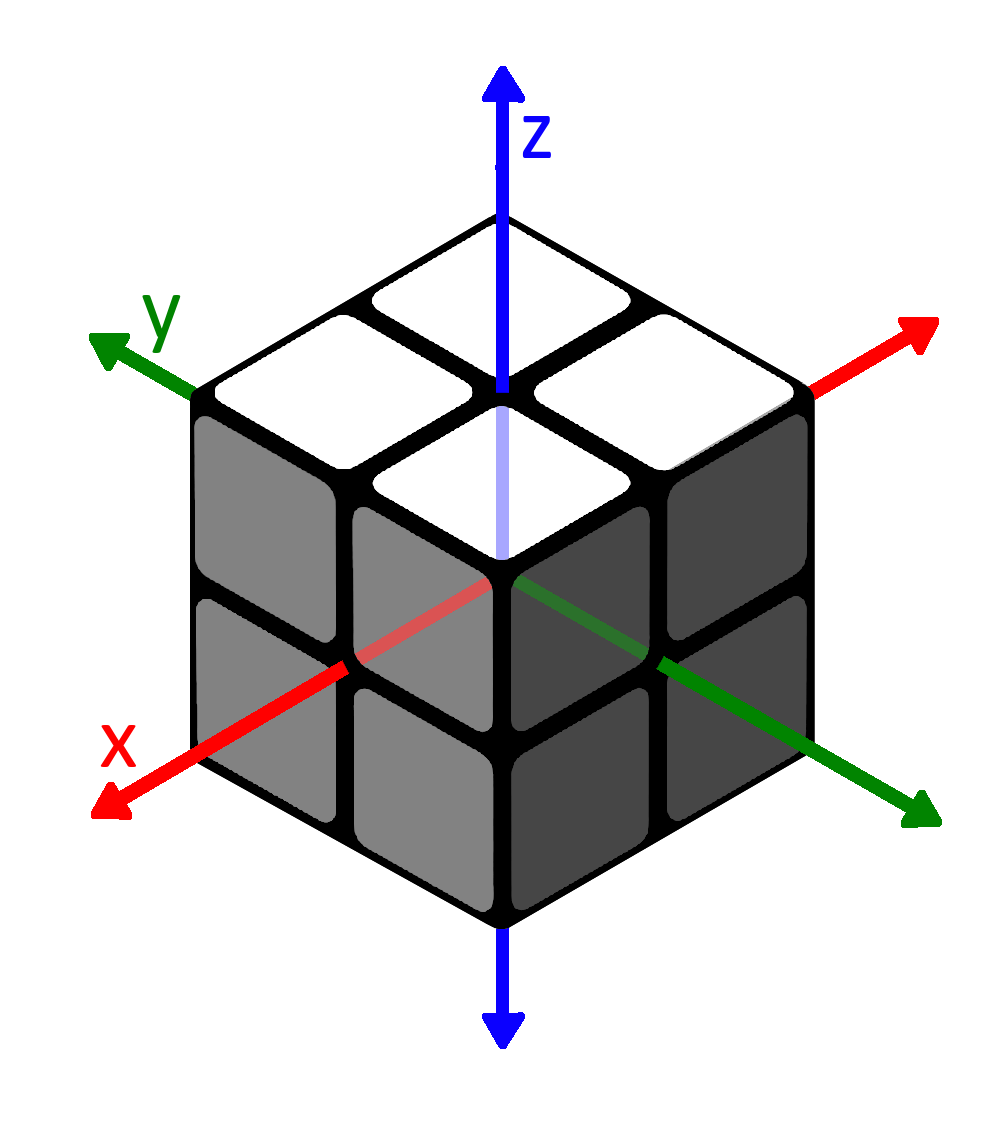
\includegraphics[scale=0.13]{Pfeile.png}
\end{figure} 
\ \\ 
\\
Nun kann ich für die möglichen Rotationen des Würfels Nachfolgekonfigurationen festlegen. \\
\\
Dazu benenne ich zuerst die einzelnen Rotationen des Würfels: \\
\\
\begin{tabular}{|c|l|}
\hline
Abkürzung & Beschreibung der Rotation \\
\hline
\hline
$Z_l$ & Rotation des Würfels um die $z$-Achse nach links (gegen den Uhrzeigersinn)\\
\hline
$Z_r$ & Rotation des Würfels um die $z$-Achse nach rechts (im Uhrzeigersinn)  \\
\hline
$Y_l$ & Rotation des Würfels um die $y$-Achse nach links (gegen den Uhrzeigersinn)\\
\hline
$Y_r$ & Rotation des Würfels um die $y$-Achse nach rechts (im Uhrzeigersinn)  \\
\hline
$X_l$ & Rotation des Würfels um die $x$-Achse nach links (gegen den Uhrzeigersinn)\\
\hline
$X_r$ & Rotation des Würfels um die $x$-Achse nach rechts (im Uhrzeigersinn) \\
\hline
\end{tabular} \\
\\
Die Steine werden durch eine Rotation alle an einen neuen Platz gebracht. Anders als bei der Drehung der Ebenen, wo nur einige Steine die Position ändern, ändern hier alle Steine die Position, ohne dass der Würfel verändert wird, da er komplett gedreht wird. \\
\\
Anhand der Rotation $Z_r$, also einer Rotation des kompletten Würfels um die $z$-Achse um $90^\circ$ im Uhrzeigersinn, zeige ich nun die Veränderung der Würfelpositionen. 
\begin{figure}[H]
\centering
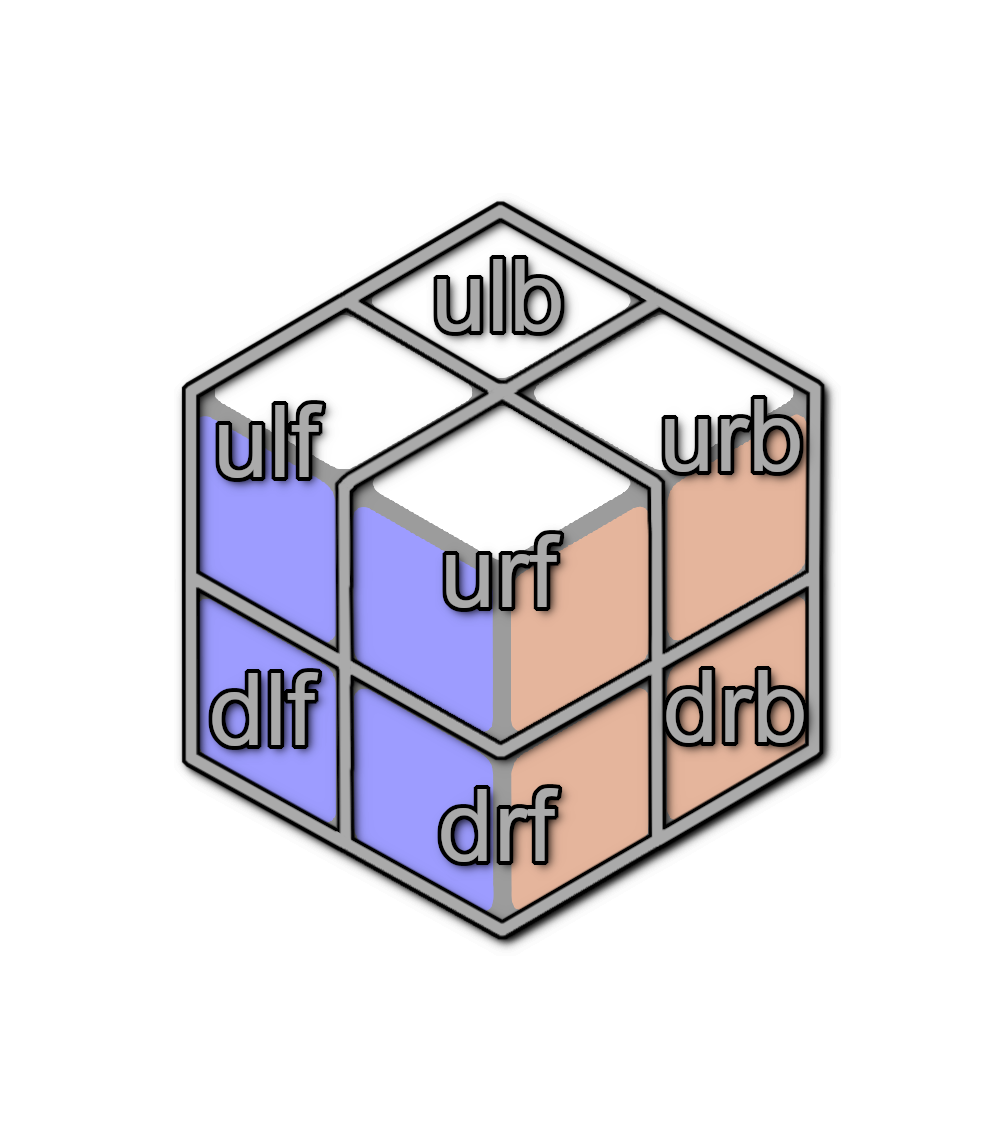
\includegraphics[scale=0.13]{auf_ulf.png}
\end{figure}
\ \\
Da bei den Rotationen alle Steine die Position wechseln, muss es 8 Funktionen $\delta$ geben, also für jeden Eckstein eine Funktion $\delta$: \\
\\
$
\delta_{Z_r}(urf) = ulf \ \ \ \ \ \ \delta_{Z_r}(ulf) = ulb \ \ \ \ \ \ \delta_{Z_r}(ulb) = urb \ \ \ \ \ \ \delta_{Z_r}(urb) = urf \\
\delta_{Z_r}(drf) = dlf \ \ \ \ \ \ \delta_{Z_r}(dlf) = dlb \ \ \ \ \ \ \ \delta_{Z_r}(dlb) = drb \ \ \ \ \ \ \delta_{Z_r}(drb) = drf
$
\\
\\
Wenn man das nun in der Form $i \mapsto j$ schreibt, erhält man: \\
\\
$urf \mapsto ulf$ \ \ \ \ \ \ \ \ $ulf \mapsto ulb$ \ \ \ \ \ \ \ \ $ulb \mapsto urb$ \ \ \ \ \ \ \ \ $urb \mapsto urf$ \\
$drf \mapsto dlf$ \ \ \ \ \ \ \ \ $dlf \mapsto dlb$ \ \ \ \ \ \ \ \ \ $dlb \mapsto drb$ \ \ \ \ \ \ \ \ $drb \mapsto drf$ \\
\\
In der Zykel-Schreibweise sieht die Veränderung der Steinnamen dann so aus: \\
$\delta_{Z_r}=(urf \ ulf \ ulb \ urb)(drf \ dlf \ dlb \ drb )$ \\
\\
Alle Rotationen sehen in Zykel-Schreibweise folgendermaßen aus:
\begin{align*}
\delta_{Z_r} & = (ulf \ ulb \ urb \ urb) \ (dlf \ dlb \ drb \ drf)\\
\delta_{Z_l} & = (ulf \ urf \ urb \ ulb) \ (dlf \ drf \ drb \ dlb)\\
\delta_{Y_r} & = (ulf \ ulb \ dlb \ dlf) \ (urf \ urb \ drb \ drf)\\
\delta_{Y_l} & = (ulf \ dlf \ dlb \ ulb) \ (urf \ drf \ drb \ urb)\\
\delta_{X_r} & = (ulf \ urf \ drf \ dlf) \ (urb \ ulb \ dlb \ drb)\\
\delta_{X_l} & = (ulf \ dlf \ drf \ urf) \ (urb \ ulb \ dlb \ drb)\\
\end{align*}
Bei den Rotationen schreibe (analog zu den Zügen) die mehrfache Ausführung einer Roatation mit der Exponentenschreibweise. \\
Somit gilt dann auch hier $RRRR=R^4=N$ (für $R \in \{{Z_r}, {Z_l}, {Y_r}, {Y_l}, {X_r}, {X_l} \}$) und $R^0=N$ (für alle Rotationen). ($N$ ist das neutrale Element, also der leere Zug und $R$ eine beliebige Rotation des Würfels.) \\
Analog zu den Zügen gilt bei den Rotationen also für jede Rotation: \\
 $\forall R \in \{{Z_r}, {Z_l}, {Y_r}, {Y_l}, {X_r}, {X_l} \}, n \in \mathbb{N} \ . \ R^n=R^{n \mod 4}$.














%=======================================================================================================













%\hspace*{2cm}

%\color{gray}


%\subsection*{Äquivalenzrelationen der Rotationen (Fehlversuch)}\addcontentsline{toc}{subsection}{\protect\numberline{}Äquivalenzrelationen der Rotationen (Fehlversuch)}


%Um die Rotationen des Würfels umzusetzen, führe ich Äquivalenzrelationen ein. \\
%Eine Relation $R \subseteq A \times A$ heißt Äquivalenzrelation auf $A$, wenn für alle $x, y, z \in A$ die drei folgenden Eigenschaften gelten: Reflexivität, Symmetrie, Transitivität. \cite{Buch} \\
%\\
%In dem Fall der Gruppe $(G_{2x2x2}, \circ)$ handelt es sich um eine Relation von zwei Zügen $Z_1, Z_2 \in G_{2x2x2}$. \\ 
%Ich führe für jede Rotationsrichtung eine Relation ein. Es gibt dann also $\sim_{Z_r}, \sim_{Z_l}, \sim_{Y_r}, \sim_{Y_l}, \sim_{X_r}, \sim_{X_l}$. \\ 


%\begin{tabular}{l l}

%$Z_1 \sim_{Z_r} Z_2$ & $:\Leftrightarrow \ \ \ \ \  Z_1$ und $Z_rZ_2$  ergeben die gleiche Würfelkonfiguration\\

%\end{tabular}
%\\
%$Z_rZ_2$ steht für den Zug $Z_2$, der nach einer Rechtsrotation des Würfels ausgeführt wird. \\
%\\
%Die anderen Rotationsrelationen definiere ich wie folgt: 

%\begin{tabular}{l l l}

%$Z_1 \sim_{Z_l} Z_2$ & $:\Leftrightarrow \ \ \ \ \  Z_1$ und $Z_lZ_2$ & ergeben die gleiche Würfelkonfiguration \\
%$Z_1 \sim_{Y_r} Z_2$ & $:\Leftrightarrow \ \ \ \ \  Z_1$ und $Y_rZ_2$ & ergeben die gleiche Würfelkonfiguration\\
%$Z_1 \sim_{Y_l} Z_2$ & $:\Leftrightarrow \ \ \ \ \  Z_1$ und $Y_lZ_2$ & ergeben die gleiche Würfelkonfiguration\\
%$Z_1 \sim_{X_r} Z_2$ & $:\Leftrightarrow \ \ \ \ \  Z_1$ und $X_rZ_2$ & ergeben die gleiche Würfelkonfiguration\\
%$Z_1 \sim_{X_l} Z_2$ & $:\Leftrightarrow \ \ \ \ \  Z_1$ und $X_lZ_2$ & ergeben die gleiche Würfelkonfiguration\\

%\end{tabular}
%\\
%\\
%\\
%\\
%Damit $\sim_{Z_r}, \sim_{Z_l}, \sim_{Y_r}, \sim_{Y_l}, \sim_{X_r}$ und $\sim_{X_l}$ Äquivalenzrelationen sind, müssen Reflexivität, Symmetrie und Transitivität gelten, was ich im folgenden Abschnitt beweise. Ich nutze das Symbol $\sim$ für alle Elemente aus  $\{ \sim_{Z_r}, \sim_{Z_l}, \sim_{Y_r}, \sim_{Y_l}, \sim_{X_r}, \sim_{X_l}\}$ und $W$ als beliebige Würfelrotation (${Z_r}, {Z_l}, {Y_r}, {Y_l}, {X_r}$ oder ${X_l}$).\\



%\begin{itemize}

%\item Reflexivität: \\
%Für die Reflexivität muss $x \sim x$ gelten. \\
%Da alle $\sim \in \{ \sim_{Z_r}, \sim_{Z_l}, \sim_{Y_r}, \sim_{Y_l}, \sim_{X_r}, \sim_{X_l}\}$ durch die Gleichheit definiert sind, gilt:
%\begin{align*}
%Z_1 \sim_W Z_2 : & \Leftrightarrow \ \ \  Z_1 \ und  \ WZ_2 \ ergeben \ die \ gleiche \ W"urfelkonfiguration\\
%& \Leftrightarrow \ \ \ C \cdot Z_1=C \cdot WZ_2 \\
%& \Leftrightarrow \ \ \ Z_1=WZ_2
%\end{align*}
%$\lightning$ Das gilt aber leider nicht, wenn $Z_1=Z_2$ gilt. Denn identische Züge ergeben nicht das gleiche, wenn der Würfel vor einem Zug rotiert wird und vor dem anderen nicht. \\
%\\


%\item Symmetrie $\lightning$%:  \\
%Für die Symmetrie muss gelten: Aus $x \sim y \ folgt \ y \sim x$. \\
%Auch das gilt, da alle $\sim \in \{ \sim_{Z_r}, \sim_{Z_l}, \sim_{Y_r}, \sim_{Y_l}, \sim_{X_r}, \sim_{X_l}\}$ durch die Gleichheit definiert sind.  

%\item Transitivität $\lightning$

%\end{itemize}

%Diese Ansatz dieser Äquivalenzrelationen funktioniert so nicht, da die Reflexivität, Symmetrie und Transitivität nicht erfüllt sind. \\ 

%falsch













% Versuch 2
%=======================================================================================================














\color{black}

\subsection*{Äquivalenzrelationen der Rotationen}\addcontentsline{toc}{subsection}{\protect\numberline{}Äquivalenzrelationen der Rotationen}

Um die Rotationen des Würfels umzusetzen, führe ich Äquivalenzrelationen ein. \\
Eine Relation $R \subseteq A \times A$ heißt Äquivalenzrelation auf $A$, wenn für alle $x, y, z \in A$ die drei folgenden Eigenschaften gelten: Reflexivität, Symmetrie, Transitivität. \cite{Buch} \\
\\
In dem Fall der Gruppe $(G_{2x2x2}, \circ)$ handelt es sich um eine Relation von zwei Zügen $Z_1, Z_2 \in G_{2x2x2}$. \\ 
\\
Ich definiere: \\  \\
\begin{tabular}{l l}
$Z_1 \sim Z_2 :\Leftrightarrow \ $  & $Z_1 \ und \ Z_2 \ ergeben \ (mit \ optionaler \ Rotation) \ die \ gleiche $\\
\  & $W"urfelkonfiguration$ \\
\end{tabular}
\\
\\
Daraus ergibt sich $Z_1 \sim Z_2 :\Leftrightarrow \ Z_1 = WZ_2$ mit $W$ als Element (oder Kombination von Elementen) aus $\{{Z_r}, {Z_l}, {Y_r}, {Y_l}, {X_r}, {X_l}, \epsilon\}$, wobei $\epsilon$ die \glqq leere\grqq \ Rotation darstellt, also keine Rotation des Würfels. \\
\\ 
Somit ergibt sich beispielsweise $F \sim L \Leftrightarrow F = Z_rL$, da eine Drehung der vorderen Ebene und eine Drehung des Würfels nach links mit einer Drehung der linken Ebene die gleiche Würfelkonfiguration ergeben. Der Würfel ist dann nur verschieden ausgerichtet. \\
\\
In der folgenden Abbildung sieht man dieses Beispiel nochmal grafisch: Links befindet sich der gelöste Würfel, in der Mitte der gelöste Würfel nach dem Zug $F$ und rechts der gelöste Würfel nach dem Zug $Z_rL$. \\
Die beiden rechten Würfel sind in der gleichen Konfigurationen, aber anders gedreht.
\begin{figure}[H]
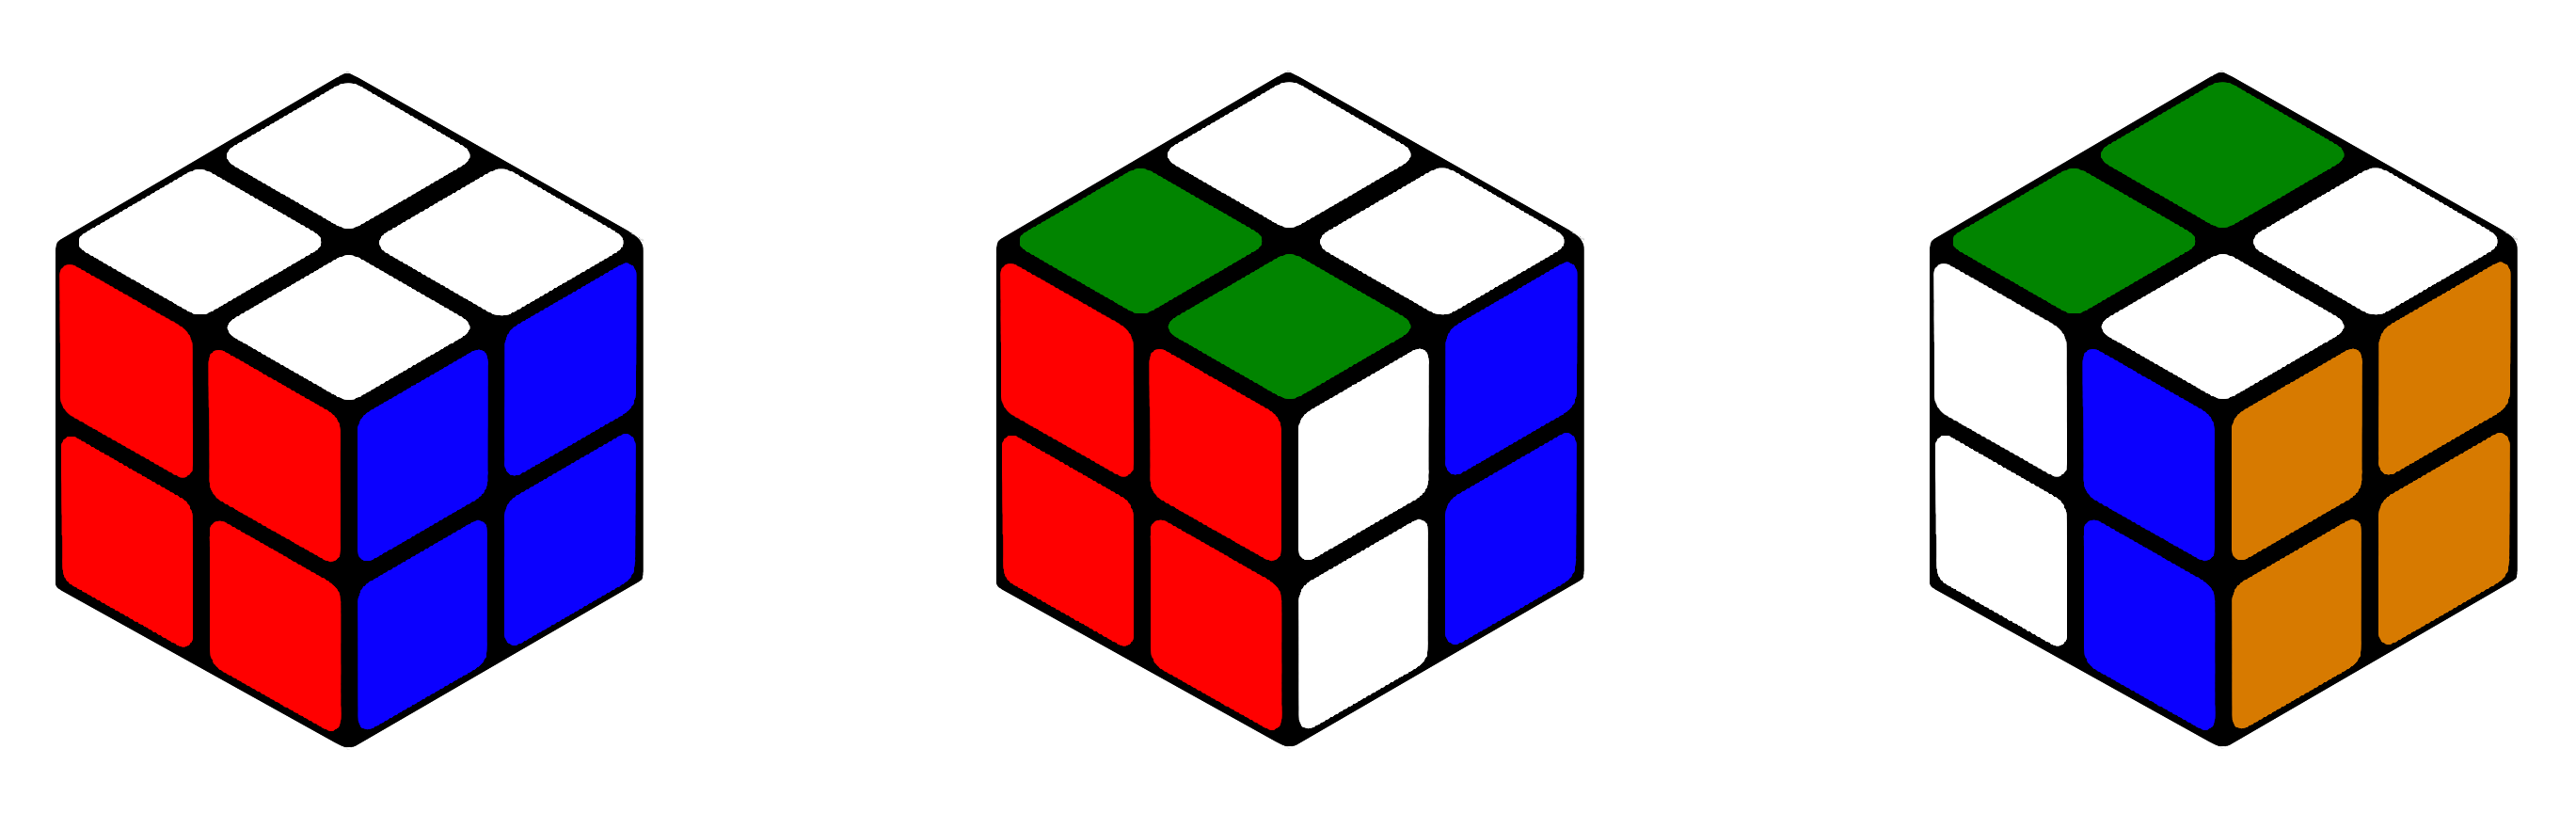
\includegraphics[scale=0.15]{3_wuerfel.png}
\end{figure}

Damit $\sim$ eine Äquivalenzrelation ist, müssen Reflexivität, Symmetrie und Transitivität gelten, was ich im folgenden Abschnitt beweise.



\begin{itemize}

\item Reflexivität:\\
Für die Reflexivität muss $Z \sim Z$ für alle $Z \in G_{2x2x2}$ gelten. 
\begin{align*}
Z_1 \sim Z_2 : & \Leftrightarrow  Z_1 = WZ_2
\end{align*}
Ich wähle $W$ als $\epsilon$, so dass keine Rotation ausgeführt wird.
\begin{align*}
Z_1 \sim Z_2 : & \Leftrightarrow  Z_1 = WZ_2 \\
\ & \Leftrightarrow Z_1=\epsilon Z_2 \\
\ & \Leftrightarrow Z_1 = Z_2
\end{align*}
Also gilt die Reflexivität für $\sim$, da für $Z_1 \sim Z_2$ mit $W=\epsilon$ immer $Z_1 = Z_2$ gilt.

\item Symmetrie: \\
Für die Symmetrie muss gelten: Aus $Z_1 \sim Z_2$ folgt $Z_2 \sim Z_1$.
\begin{align*}
Z_1 \sim Z_2 & \Rightarrow Z_2 \sim Z_1 \\
mit \ Z_1 \sim Z_2 : & \Leftrightarrow  Z_1 = WZ_2 \\
\Leftrightarrow Z_1 = W_1 Z_2 & \Rightarrow Z_2 = W_2 Z_1
\end{align*}
Das gilt, wenn $W_2$ das Inverse von $W_1$ ist. Das Inverse ist die Rotation um die gleiche Achse, aber in die andere Richtung. \\
Ich schreibe das Inverse von $W$ als $W^{-1}$. \\

Das sind die Rotationen mit den dazugehörigen Inversen: \\

\begin{tabular}{|l||c|c|c|c|c|c|c|}
\hline
Rotation $W$ & ${Z_r}$ & ${Z_l}$ &  ${Y_r}$ & ${Y_l}$ & ${X_r}$ & ${X_l}$ & $\epsilon$ \\
\hline
Inverses $W^{-1}$ & ${Z_l}$ & ${Z_r}$ &  ${Y_l}$ & ${Y_r}$ & ${X_l}$ & ${X_r}$ & $\epsilon$ \\
\hline
\end{tabular} \\
\\
Dann gilt: 
\begin{align*}
Z_1 = W Z_2 & \Rightarrow Z_2 = W^{-1} Z_1
\end{align*}
Das gilt, da durch $W^{-1}$ der Würfel in die entgegengesetzte Richtung rotiert wird und die Züge somit wieder die gleiche Würfelkonfiguration ergeben. \\
Also gilt die Symmetrie für $\sim$.


\item Transitivität: \\
Es muss gelten: Aus $Z_1 \sim Z_2$ und $Z_2 \sim Z_3$ folgt $Z_1 \sim Z_3$.
\begin{alignat*}{3}
& Z_1 \sim Z_2 && \wedge Z_2 \sim Z_3 && \Rightarrow Z_1 \sim Z_3 \\
\Leftrightarrow \ & Z_1 = W_1Z_2 \ && \wedge Z_2 = W_2Z_3 \ && \Rightarrow Z_1 = W_3Z_3
\end{alignat*}
Das gilt, für $W_3=W_1W2$.
\begin{alignat*}{3}
\Leftrightarrow \ & Z_1 = W_1Z_2 \ && \wedge Z_2 = W_2Z_3 \ && \Rightarrow Z_1 = W_1W_2Z_3 
\end{alignat*}
Da die Züge $Z_1$ und $Z_2$ mit der Rotation $W_1$ die gleiche Würfelkonfiguration ergeben, und die Züge $Z_2$ und $Z_3$ nach der Rotation $W_2$ auch die gleiche Würfelkonfiguration ergeben, gilt das auch für die beiden Züge $Z_1$ und $Z_3$ nach der Rotation $W_3=W_1W_2$, da dann alle nötigen Rotationen durchgeführt wurden.

\end{itemize}








%=======================================================================================================













\subsection*{Ordnung der Züge}\addcontentsline{toc}{subsection}{\protect\numberline{}Ordnung der Züge}
Wie bereits beschrieben, gilt $\forall Z \in \{ U, D, F, B, L, R \}, n \in \mathbb{N} \ . \ Z^n=Z^{n \mod 4}$ für alle einelementigen Züge (und Rotationen), da alle Steine des Würfels in ihrer vorherigen Position bleiben, wenn eine Ebenen- oder eine Würfelrotation vier mal hintereinander ausgeführt wird. Deshalb bezeichne ich die Züge $U, D, F, B, L, R$ als Züge der Ordnung 4. \\
\\
Die Exponentenschreibweise kann man für alle Züge aus $G_{2x2x2}$ anwenden, auch wenn sie mehr als eine Ebene rotieren. Beispielsweise mit $Z_1=LLFF$. $(LLFF)^2$ ist dann $LLFFLLFF$ und $(LLFF)^3$ ist $LLFFLLFFLLFF$, was wieder die Ausgangsposition ergibt. \\
\\
Nicht nur die Züge $U, D, F, B, L, R$ kommen nach Wiederholen in den Ausgangszustand. Auch alle anderen Züge bringen den Würfel wieder in die Ausgangsposition des Zuges \cite{TD}. Es sind aber je nach Zug verschieden viele Wiederholungen nötig. Der Zug $(LLFF)$ hat dann beispielsweise die Ordnung 3. \\
So gilt zum Beispiel: ${R^4= N}$ (Ordnung 4), ${(RRFF)^3 = N}$ (Ordnung 3) oder auch ${(LF)^{15}=N}$ (Ordnung 15).\\ Dabei muss beachtet werden, dass die Ordnung die Anzahl der Durchführungen beschreibt, die benötigt wird, damit alle Steine wieder an der Ausgangsposition sind. Die Ausrichtung der Steine wird hier aber nicht berücksichtigt. \\
\\
Im folgenden Beweis habe ich mich an dem Beweis aus dem Paper \glqq Group Theory via Rubik's Cube\grqq \ von Tom Davis \cite{TD} orientiert: \\
Jedes Mal wenn ein Zug wiederholt wird, werden die Steine im Würfel neu angeordnet. \\ 
Da es eine endliche Anzahl an Würfelkonfigurationen gibt, muss eine Würfelposition wiederholt werden, wenn man den Zug oft genug durchführt. \\
Die Zahl der validen Würfelkonfigurationen ist zwar sehr groß, aber endlich. Also muss eine Position wiederholt werden, wenn man den Zug öfter ausführt, als es mögliche Würfelpositionen gibt. \\
\\
Bei einem beliebigen Zug $Z \in G_{2x2x2}$ gelangt man also irgendwann in eine Würfelposition, die sich wiederholt. Die wiederholende Würfelposition tritt zuerst nach $n \in \mathbb{N}$ Wiederholungen auf und das zweite Mal nach $m \in \mathbb{N}$ Wiederholungen. Das sieht dann so aus: $Z^n=Z^m$ mit $n < m$. \\
\\
Also gilt $Z^{n-1} \neq Z^{m-1}$, da $m$ das zweite Vorkommen der gleichen Position repräsentiert. \\
Wenn $n=0$ ist, hat man $Z^0=N$, was den leeren Zug (bzw. das neutrale Element) repräsentiert. Der Würfel wird dabei nicht verändert und somit wird die Würfelposition bei jedem Zug $Z \in G_{2x2x2}$ mit $Z^0$ \glqq wiederholt\grqq . \\
\\
Es gilt $Z^n = Z^m$. Wenn man nun auf die gleiche Ausgangsposition $n$-mal oder $m$-mal $Z$ anwendet, kommt man in der gleichen Endposition an. \\
Wenn man nun $Z^{-1}$ anwendet, kommt man wieder in die gleiche Endposition. Dabei ist es egal, ob man vorher $n$-mal oder $m$-mal $Z$ ausgeführt hat, da man von der gleichen Startposition ausgehend in die gleiche Endposition kommt, wenn man den gleichen Zug ausführt. \\
\\
Beim Anwenden von $Z^{-1}$ wird die letzte Ausführung von $Z$ wieder rückgängig gemacht. Wenn man $Z$ also $n$-mal ausführt und dann $Z^{-1}$ ausführt, ist es das gleiche wie $n-1$-mal $Z$ ausführen, also $Z^nZ^{-1}=Z^{n-1}$. Das gilt natürlich auch für $m$, also $Z^mZ^{-1}=Z^{m-1}$. \\
\\
Demnach gilt dann $Z^{n-1}=Z^{m-1}$. Das widerspricht dann aber der Annahme, dass $m$ der kleinste Wert für eine Wiederholung der Position ist. Also muss $n=0$ sein, damit $m$ die erste Wiederholung einer Position repräsentiert. \\
\\
Daraus folgt: Wenn man einen beliebigen Zug $Z \in G_{2x2x2}$ wiederholt auf den gelösten Würfel anwendet, kommt man wieder in die Startkonfiguration.
 












%=======================================================================================================









\newpage


\subsection*{Zykelstruktur}\addcontentsline{toc}{subsection}{\protect\numberline{}Zykelstruktur}


Anhand der Zykelstruktur lässt sich die Ordnung des jeweiligen Zuges bestimmen. Die Ordnung beschreibt die Anzahl der Wiederholungen, die ein Zug durchgeführt werden muss, damit die Steine die gleiche Anordnung wie zu Beginn des Zuges haben. Dabei geht es um die Steinpositionen und nicht um die Steinausrichtungen.\\
Der Würfel kann also alle Steine an der richtigen Position haben und trotzdem ungelöst sein, da die Steine verdreht sein können. \\
\\
Der Zug $U$ als $\sigma_U =\ (ulf \ ulb \ urb \ urf) $ (eine Drehung der oberen Ebene um $90^\circ$ im Uhrzeigersinn) besteht aus einem 4-elementigen Zykel. \\
Wenn der Zug $U$ also viermal ausgeführt wird, befindet sich der Würfel wieder in seiner vorherigen Position: \\ \\
\begin{tabular}{|c||c|c|c|c|}
\hline
Ausführung & ulf & ulb & urb & urf \\
\hline
\hline
1 & ulb & urb & urf & ulf \\
\hline
2 & urb & urf & ulf & ulb \\
\hline
3 & urf & ulf & ulb & urb \\
\hline
4 & ulf & ulb & urb & urf \\
\hline

\end{tabular}
\ \\
\\
Die vierte Zeile der Tabelle hat die selbe Anordnung der Steine wie die oberste Zeile (vor Ausführung von $U$). \\
Somit hat die beschriebene Ebenenrotation $U$ die Ordnung 4. Das gilt auch für jede andere Ebenenrotation ($D, F, B, L, R$).\\
\\
Es gilt also für einen Zug $Z$, der aus nur einem $n$-elementigen Zykel besteht: \\ 
${\forall \ Z \in G_{2x2x2}\ mit \ Z=(i_1 \ i_2 \ ... \ i_n), n \in \mathbb{N} \ . \  Z^n=1 }$. \\
\\
Wenn man $Z$ mehrfach ausführt, kommt man nach jeder $n$-ten Wiederholung in den Ausgangszustand. \cite{TD} Es gilt also auch 
${\forall \ Z \in G_{2x2x2}\ mit \ Z=(i_1 \ i_2 \ ... \ i_n), n,k \in \mathbb{N} \ . \  Z^{k*n}=1 }$.
\\
\\
Auch bei komplexeren Zügen kann anhand der Zykelstruktur die Ordnung bestimmt werden. Dazu muss das $KGV$ (kleinstes gemeinsames Vielfaches) aller Zykelgrößen bestimmt werden. \cite{TD}
\\
\\
\newpage 
Der besseren Übersichtlichkeit halber, habe ich die Zykel aller Züge auch grafisch dargestellt:

\begin{figure}[H]
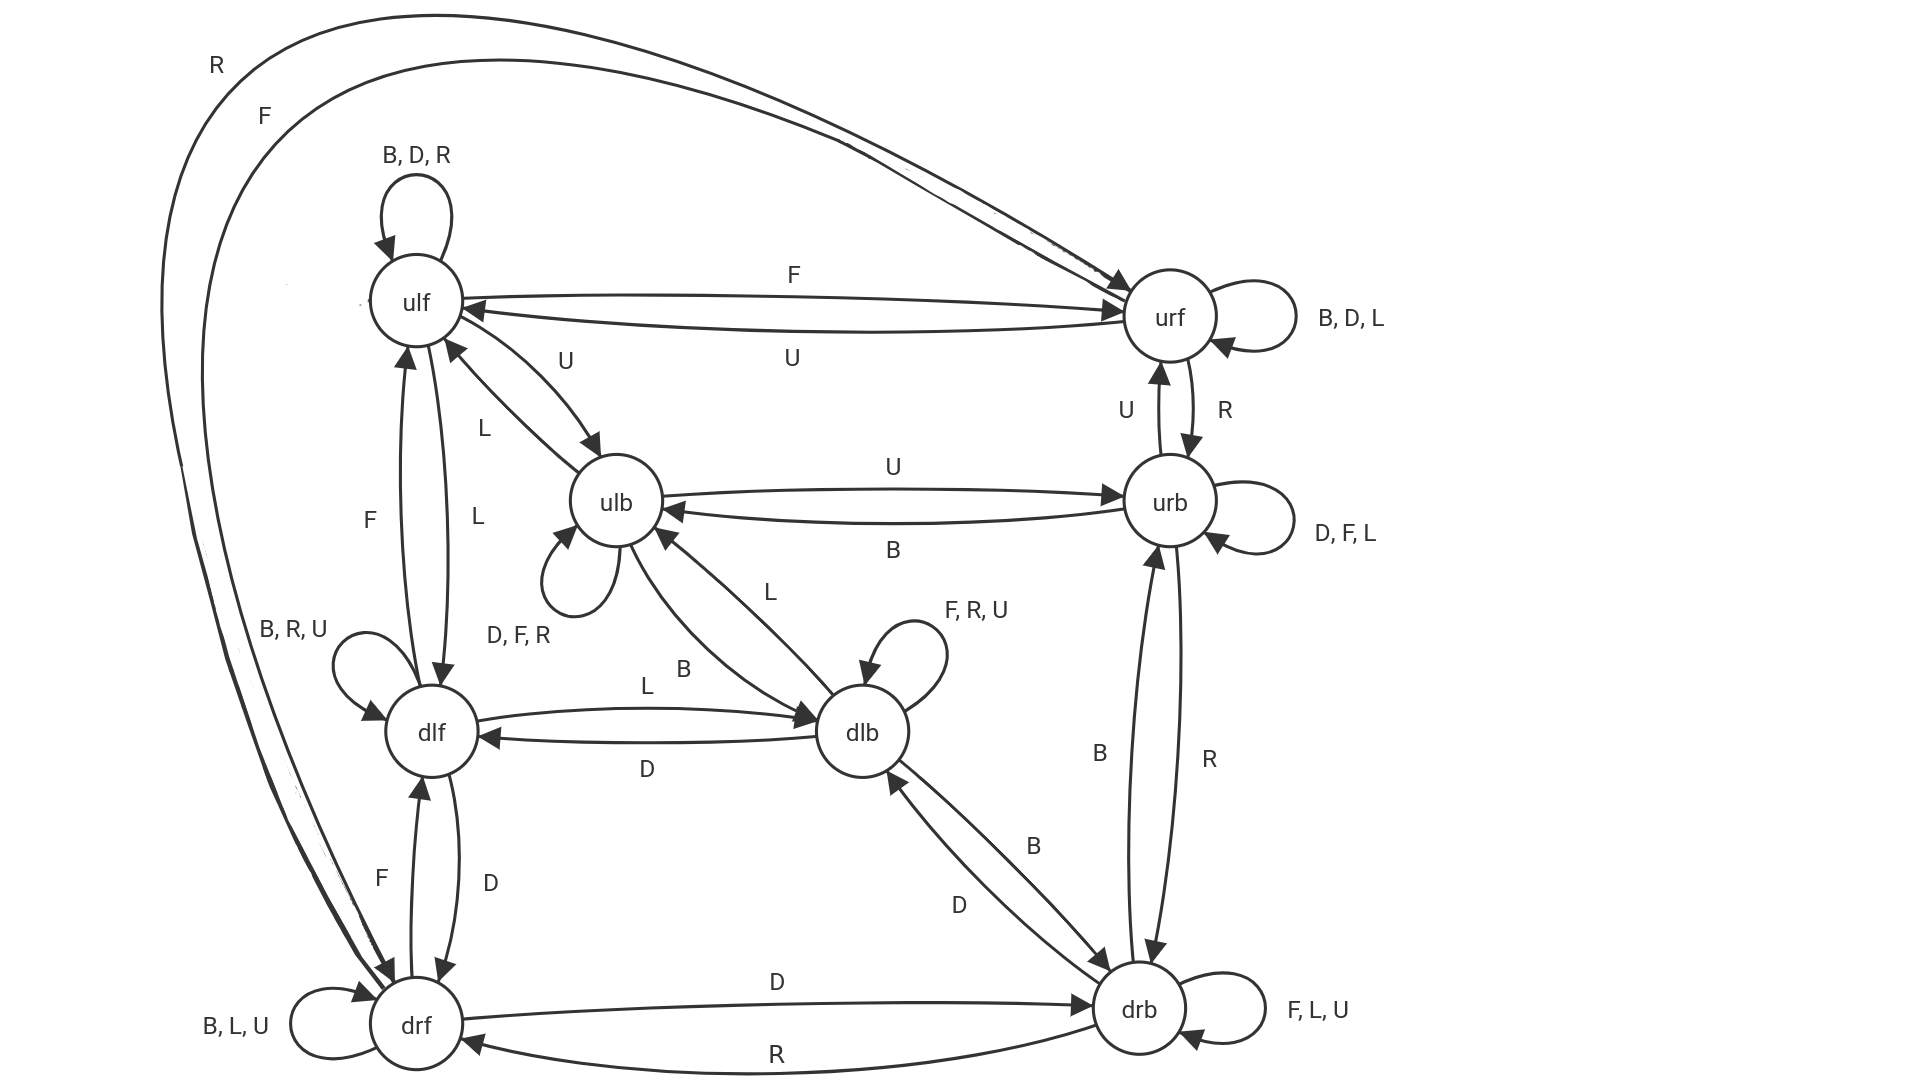
\includegraphics[scale=0.3]{graph_zug.png}
\end{figure}
\ \\
Dieser Graph vereinfach das Ablesen der Zykel, vorallem wenn bei einem Zug mehrere Ebenenrotationen kombiniert werden. \\
\\
So kann ich nun anhand des Beispielzuges $LLFF$ die Zykelstruktur darstellen. \\
\\
Zuerst erstelle ich eine Tabelle, die jede Position auf ihre neue Position abbildet. \\
\\
\begin{tabular}{|c||c|c|c|c|c|c|c|c|}
\hline
 & ulb & urb & ulf & urf & dlb & drb & dlf & drf \\
\hline
\hline
L & ulf & \textcolor{gray}{urb} & dlf & \textcolor{gray}{urf} & ulb & \textcolor{gray}{drb} & dlb & \textcolor{gray}{drf} \\
\hline
L & dlf & \textcolor{gray}{urb} & dlb & \textcolor{gray}{urf} & ulf & \textcolor{gray}{drb} & ulb & \textcolor{gray}{drf} \\
\hline
F & ulf & \textcolor{gray}{urb} & \textcolor{gray}{dlb} & drf & urf & \textcolor{gray}{drb} & \textcolor{gray}{ulb} & dlf \\
\hline
F & urf & \textcolor{gray}{urb} & \textcolor{gray}{dlb} & dlf & drf & \textcolor{gray}{drb} & \textcolor{gray}{ulb} & ulf \\
\hline

\end{tabular}
\ \\ \\ \\
Die ausgegrauten Positionen bleiben bei dem jeweiligen Zug unverändert. \\
\\ \\
\\
Grafisch dargestellt sehen die Zykel des Zuges $LLFF$ so aus: \\
\begin{figure}[H]
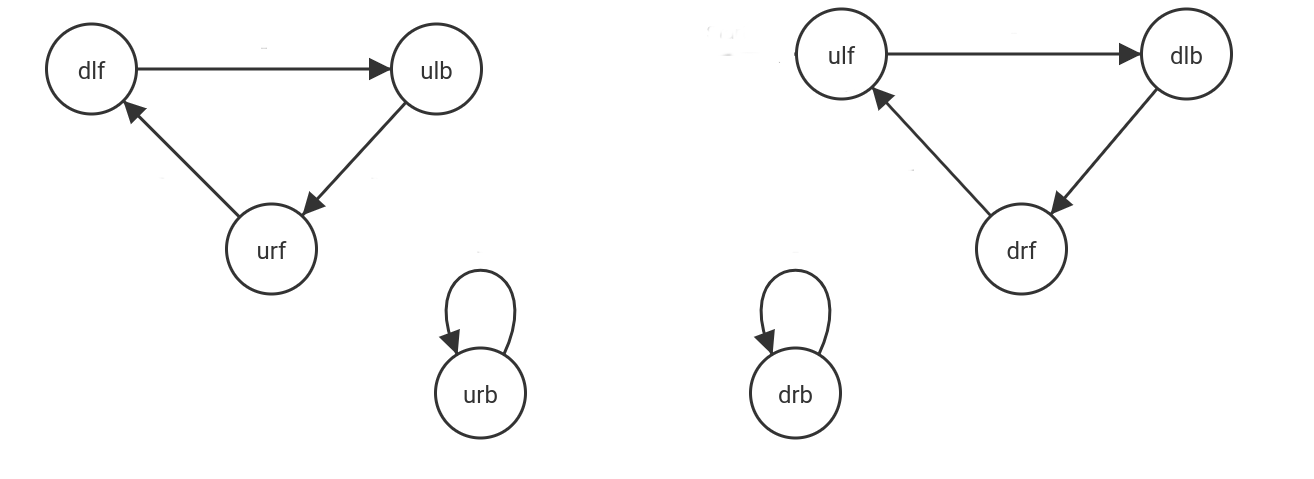
\includegraphics[scale=0.3]{zykel_LLFF.png}
\end{figure}

In Zykelschreibeweise also $\sigma_{LLFF}=(dlf \ ulb \ urf)(ulf \ dlb \ drf)$. \\
Da es also zwei Zykel der Länge drei gibt, befinden sich alle Würfelsteine nach drei Zügen ($KGV(3,3,1,1)=3$) wieder in ihrer Ausgangsposition. \\
In diesem Fall sind die Steine nicht nur an der richtigen Position sondern auch so ausgerichtet, wie zu Beginn des Zuges. \\
\\
Außerdem kann man erkennen, dass sechs der acht Steine bei dem Zug $LLFF$ bewegt werden. Die anderen beiden ($urb$ und $drb$) bleiben unverändert. \\
\\













%=======================================================================================================













\subsection*{Äquivalenz von Zügen}\addcontentsline{toc}{subsection}{\protect\numberline{}Äquivalenz von Zügen}


Es kann schwierig sein, die Äquivalenz von Zügen oder Roatationen anhand der Funktionen ($\sigma$ und $\delta$) in der Zykelschreibweise zu erkennen. \\
Das liegt daran, dass man die Zykel in verschiedener Reihenfolge schreiben kann. So ist der Zug $U$ beispielsweise $ (ulf \ ulb \ urb \ urf)$, aber auch $(urb \ urf \ ulf \ ulb)$.
\\
Um das zu vereinfachen, priorisiere ich die Würfelpositionen, so dass die Position mit der höchsten Priorität immer vorne steht und zwei Äquivalente Zykel somit gleich aussehen. \\
\\
Die Positionen priorisiere ich wie folgt: \\ \\
\begin{tabular}{|c||c|c|c|c|c|c|c|c|}
\hline
Priorität & 1 & 2 & 3 & 4 & 5 & 6 & 7 & 8 \\
\hline
Position  & ulb & urb & ulf & urf & dlb & drb & dlf & drf \\
\hline
\end{tabular}
\ \\ \\ \\
Somit ist die angepasste Schreibweise für den Zug $U$ dann $(ulb \ urb \ urf \ ulf)$, da $ulb$ (falls vorhanden) ganz vorne stehen muss.














%=======================================================================================================








\newpage

\section{Untergruppen von G$_{2x2x2}$}


Eine Gruppe $(H, \circ)$, ist eine Untergruppe einer Gruppe $(G, \circ)$, wenn $H \subseteq G$ gilt. \\
Dann schreibt man auch $H \leqslant G$. \\
Das Symbol $\leqslant$ ist zu lesen als \glqq ist Untergruppe von\grqq. \\
\\
Jede Gruppe G mit neutralem Element $N$ hat die beiden trivialen Untergruppen ${H_N = \{N\}}$ und $H_G=G$ (hier: $G_2=G_{2x2x2}$). Also sind $H_N$ und $H_G$ die trivialen Untergruppen von $G_{2x2x2}$. ($H_N \leqslant G_{2x2x2}$ und $H_G \leqslant G_{2x2x2}$)\\
Die Gruppe $G_{2x2x2}$ hat viele Untergruppen, deshalb kann ich nur auf einen Teil davon eingehen. \\
\\
Da die trivialen Untergruppen nicht sonderlich interessant sind, gehe ich im folgenden Abschnitt auf einige anschauliche Untergruppen zum Lösen des Würfels ein. Diese Gruppen hat Tom Davis (in seinem Paper \glqq Group Theory via Rubik's Cube\grqq) \cite{TD} für den 3x3x3-Würfel genannt. Ich übertrage zwei seiner Untergruppen hier auf den 2x2x2: \\ 
\\
Die Untergruppe $H_{E1}$, die nur die Rotation einer Ebene zulässt, hat nur vier erreichbare Würfelkonfigurationen (sowohl beim 2x2x2- als auch beim 3x3x3-Würfel). Das kann man auch gut an einem \textit{Cube} nachvollziehen, da man durch das Drehen von nur einer Ebene auch nur vier verschiedene Ergebnisse erzielen kann. \\
\\
Eine weitere Untergruppe von $G_{2x2x2}$ ist $H_{E2}$. Hier dürfen zwei gegenüberliegende Ebenen gedreht werden. \\
Bei der Gruppe des 3x3x3-Würfels ergeben sich daraus 16 mögliche Würfelkonfigurationen \cite{TD}. Bei dem 2x2x2-\textit{Cube} allerdings nur vier, da es nur zwei Ebenen gibt und man nicht anhand der Mittelsteine oben und unten unterscheiden kann. \\
\\














%=======================================================================================================














\newpage

\section{Valide Konfigurationen des Würfels}














%=======================================================================================================













\subsection*{Ausrichtung der Steine (modulo 3)}\addcontentsline{toc}{subsection}{\protect\numberline{}Ausrichtung der Steine (modulo 3)}

Die Konfiguration des Würfels ist definiert als $C=(\sigma, x)$. \\
\\
In diesem Abschnitt werde ich zeigen, dass bei einer validen Würfelkonfiguration ${\Sigma \ x_i \mod 3 = 0}$ (modulo) gilt. \\
Wenn $C'=(\sigma', x')$ eine Nachfolgekonfiguration von $C=(\sigma, x)$ ist, dann gilt  ${(\sigma, x) \cdot M = (\sigma', x')}$. Dabei ist $M$ eine der Züge aus $U, D, R, L, F, B$. Es gilt dann ${\Sigma \ x_i' \mod 3 = \Sigma \  x_i \mod 3 }$. \\
In Abbildung 6 (s.o.) kann ist diese Situation für den Zug $R$ dargestellt. Das kann man auch anhand dieser Tabelle sehen: \\
\\
\begin{tabular}{|c|l|l|c|c|}
\hline
Zug $M$ & $x$ & $x'$ & $\Sigma \  x_i'$ & $\Sigma \  x_i' \mod 3 = 0$ \\
\hline
\hline
\textit{D} & $(x_1, x_2, x_3, x_4, x_5, x_6, x_7, x_8)$ & $(x_1, x_2, x_3, x_4, x_6, x_8, x_5, x_7)$ & 0 & 0 \\
\hline
\textit{U} & $(x_1, x_2, x_3, x_4, x_5, x_6, x_7, x_8)$ & $(x_3, x_1, x_4, x_2, x_5, x_6, x_7, x_8)$ & 0 & 0 \\
\hline
\textit{R} & $(x_1, x_2, x_3, x_4, x_5, x_6, x_7, x_8)$ & $(x_1, 2, x_3, 1, x_5, 1, x_7, 2)$ & 6 & 0 \\
\hline
\textit{L} & $(x_1, x_2, x_3, x_4, x_5, x_6, x_7, x_8)$ & $(1, x_2, 2, x_4, 2, x_6, 1, x_8)$ & 6 & 0 \\
\hline
\textit{F} & $(x_1, x_2, x_3, x_4, x_5, x_6, x_7, x_8)$ & $(x_1, x_2, 1, 2, x_5, x_6, 2, 1)$ & 6 & 0 \\
\hline
\textit{B} & $(x_1, x_2, x_3, x_4, x_5, x_6, x_7, x_8)$ & $(2, 1, x_3, x_4, 1, 2, x_7, x_8)$ & 6 & 0 \\
\hline

\end{tabular}
\ \\ 
Für jede valide Würfelposition gilt also ${\Sigma \ x_i' \mod 3 = \Sigma \  x_i \mod 3 }$. \\
\\
Wenn es also eine valide Konfiguration $C'=(\sigma', x')$, für die gilt $\Sigma x_i' \mod 3 = 0$, dann gibt es einen Zug $M \in G_{2x2x2}$, so dass $M \cdot C'$ die Steine in die richtigen Positionen bringt also $(1,x)$. \\
\\
Von dieser Konfiguration $(1,x)$ ausgehend gibt es einen Zug $M \in G_{2x2x2}$, so dass alle Eckstücke richtig ausgerichtet sind. Dann ergibt sich die Konfiguration $(1, 0)$ und alle Eckstücke sind in der richtigen Ausrichtung und Position. Der Würfel befindet sich also in der Startkonfiguration. \\ 














%=======================================================================================================









\newpage


\section{Lösung des Würfels}

Die \glqq übliche\grqq \  Methode zum Lösen eines Zauberwürfels ist das Kombinieren verschiedener Ebenendrehungen. Diese werden als eine Einheit angewendet und verändern den Würfel dann sehr spezifisch. \\
Es gibt beispielsweise eine Kombination, die 3 der 4 Ecken der oberen Ebene untereinander im Uhrzeigersinn tauscht und deren Ausrichtung dabei nicht verändert. \\
\\














%=======================================================================================================













\subsection*{Parität}\addcontentsline{toc}{subsection}{\protect\numberline{}Parität}














%=======================================================================================================













\newpage



\section{Abbildungen und Tabellen}

Alle verwendeteten Grafiken, Abbildungen und Tabellen habe ich selbst (mit GIMP, Photoshop oder LateX) erstellt, um Markennennungen zu vermeiden und eine einheitliche Darstellung zu gewährleisten.



\printbibliography












\end{document}














